\documentclass[a4paper]{article}
\usepackage[utf8]{inputenc}
\usepackage[italian]{babel}

\usepackage{tabularx}
\usepackage{natbib}
%\usepackage[demo]{graphicx}
\usepackage{graphicx}

%\usepackage[margin=1.0in]{geometry}

\usepackage{hyperref} %per i link
\usepackage{tikz}
\usepackage{comment}
\usepackage{subfigure}
\usepackage{subcaption}
\usepackage{caption}
\usepackage{subfloat}
\usepackage{amsmath, amsthm}

\usepackage{mathrsfs}

\usepackage{pgfplots}
\pgfplotsset{compat=1.18}
\usepackage{caption}

\theoremstyle{definition}
\newtheorem{rich}{richiamo matematico}[section]


%roba che crea comando per centrare immagine dentro immagine piu grande
%https://tex.stackexchange.com/a/308286
\newlength{\imagew}
\newlength{\imageh}
\newlength{\legendw}
\newlength{\legendh}
\newlength{\legendx}
\newlength{\legendy}
\newcommand{\graphicswithlegend}[6]{
	\setlength{\imagew}{#1}
	\settoheight{\imageh}{\includegraphics[width=\imagew]{#2}}
	
	\setlength{\legendw}{#3\imagew}
	\settoheight{\legendh}{\includegraphics[width=\legendw]{#4}}
	
	\setlength{\legendx}{\imagew}
	\addtolength{\legendx}{-\legendw}
	\addtolength{\legendx}{-#5\imagew}
	
	\setlength{\legendy}{\imageh}
	\addtolength{\legendy}{-\legendh}
	\addtolength{\legendy}{-#6\imageh}
	
	\includegraphics[width=\imagew]{#2}%
	\llap{
		\hspace{-\the\legendx}
		\raisebox{\legendy}{\includegraphics[width=\legendw]{#4}}
		\hspace{\the\legendx}
	}
}


\title{Circuiti 2}
\date{Laboratorio di fisica II}
\author{Diana Broggi, Giulia Cantarini, Paolo Falconelli}


\begin{document}

\maketitle
\tableofcontents

\section{Introduzione}
Questa esperienza è stata svolta al fine di comprendere il funzionamento dei circuiti RC, RL e RCL sollecitati da corrente impulsata tramite la misura della differenza di potenziale ai capi dei suddetti elementi circuitali. \\

\section{Strumentazione}
Gli strumenti adoperati per la creazione ed il monitoraggio dei fenomeni interessati sono elencati di seguito \\

\begin{itemize}
    \item generatore di funzioni d'onda, utilizzato per produrre un segnale di tensione ad onda quadra; resistenza interna di 671\(\pm\) 1 \(\Omega\).
    \item oscilloscopio, permette di visualizzare l'andamento temporale del segnale ricevuto dalle sonde, e di effettuare le  misure necessarie del caso attraverso i cursori sullo schermo; reistenza interna \(\approx\) 1 \(M\Omega\) e capacità di ingresso di 20pF.
    \item cavi coassiali con conettori VNC, utilizzati per trasmettere il segnale dal generatore all'oscilloscopio, la principale caratteristica è la schermatura contro fattori di disturbo esterni; reistenza dell'ordine dei 50\(\Omega\).
    \item sonde compensate a 10x con connettore VNC in coda, adoperate per misurare la tensione in determinati punti del circuito e riferirla in ingresso all'oscilloscopio.
    \item breadboard, munita di piste conduttive e di due boccole per l'alimentazione.
     \item multimetro palmare, strumento in grado di misurare diverse grandezze, abbiamo limitato il suo utilizzo alla valutazione delle resistenze di carico e alla stima della capacità dei condensatori; sensibilità variabile. 
    \item scatola delle resistenze variabili; con resistenza interna di 0.2\(\Omega\) ed errore relativo dell'1\% sul valore segnalato.
    \item condensatori con capacità che variano dall'ordine dei nF ai \(\mu\)F.
    \item induttori di induttanza dell'ordine dei mH.
  
\end{itemize}

\section{Parte prima}
La prima parte dell'esperienza riguarda i fenomeni di carica e scarica nei circuiti RC e RL, l'alimentazione a corrente impulsata simula l'alternarsi della chiusura del circuito su un generatore di tensione e poi su un cortocircuito. \\
Il generatore è stato impostato su una frequenza di \(f = 10.000 \pm 0.001\) Hz e una differenza di potrenziale picco-picco Vpp = \(2.000 \pm 0.001\)V per tutta la duranta dell'esperimento.

\subsection{Obiettivi e metodo adottato}
L'obiettivo dell'esperienza consiste nell'osservare la risposta del circuito, in termini di intensità di corrente al suo interno, a seguito di un impulsivo aumento o diminuizione di tensione. \\
Il metodo applicato per RC è analogo anche per i circuiti successivi, con la differenza che questi possono presentare un L oppure L e C assieme. \\
Abbiamo posto le sonde collegate all'oscilloscopio ai capi della resistenza, poichè, per la legge di Ohm, la tensione ai capi di R è proporzionale alla corrente che scorre nel circuito tramite una costante a noi nota, ovvero R.\\
Per quanto riguarda RC ed RL, è interessante osservare anche l'andamento del potenziale ai capi del condensatore (o dell'induttore), oltre a quello della resistenza, per poter avere un quadro completo del fenomeno interessato; perciò abbiamo campionato nel tempo la ddp anche ai capi di C ed L. \\

\noindent Per studiare la carica del condensatore è necessario misurare l'andamento della corrente nel tempo a partire dal momento in cui comincia un picco dell'onda quadra che è in entrata nel circuito.\\
Per studiare la scarica basta posizionarsi in corrispondenza di un ventre, oppure impostare la tensione generata a -Vpp e procedere analogamente al caso precedente. Ci aspettiamo che la scarica del circuito sia un fenomento dettato da leggi simmetriche rispetto a quelle della carica; perciò, essendoci trovati in mancanza di tempo per eseguire tutte le misure richieste per l'esperienza, abbiamo deciso di concentrarci solo sul primo fenomeno. \\

\subsection{Circuito RC}

Abbiamo avviato l'esperienza costruendo un circuito RC alimentato da corrente impulsata adoperando una resistenza \(R = 0.989 \pm 0.001 k\Omega\) e un condensatore \(C = 2.42 \pm 0.01 \mu F\). 

\noindent Lo schema e la realizzazione del primo circuito sono riportati in Figura \ref{fig:RC_schema} e in Figura \ref{fig:RC_foto}:

\begin{figure}[!ht]

	\makebox[1 \textwidth][c]{       %centering table
		\resizebox{0.7 \textwidth}{!}{   %resize table
			\includegraphics{prima parte/schemaRC.png}
		} %close resize
	} %close centering
	\caption{schema di un circuito RC}

    \label{fig:RC_schema}

\end{figure}

\begin{figure}[!h]
\hfill
\subfigure[collegamento del circuito a generatore e oscilloscopio]{\includegraphics[width=6cm]{prima parte/RC_foto2.png}}
\hfill
\subfigure[misura ddp in entrata e ai capi del condensatore attraverso le sonde]{\includegraphics[width=5cm]{prima parte/RC_foto.png}}
\hfill
\caption{realizzazione in laboratorio}
\label{fig:RC_foto}
\end{figure}

\noindent La misura della differenza di potenziale ai capi di R è stata effettuata con un circuito CR, il cui schema corrispondente a quello in Figura \ref{fig:RC_schema} con R e C invertite. \\

\subsubsection*{Dati raccolti}
A partire dal tempo t = 0 (primo picco della quadra), abbiamo campionato i grafici ottenuti per la tensione ai capi di R e di C nel tempo attraverso i cursori dell'oscilloscopio, il quale mostrava a schermo valori e unità di misura del segnale ricevuto nell'istante selezionato. \\

\noindent Per ogni punto abbiamo riportato le due misure per V tra cui il valore segnalato variava, si noti che l'incertezza dello strumento stimata è pari a 2mV per il voltaggio e 0.02 ms per i tempi.

\begin{table}[!htbp]

    \captionsetup{labelformat=empty}

    \caption{Tabella1: circuiti RC e CR in carica}
\resizebox{13cm}{!}{

    \begin{minipage}{.5\linewidth}
      \caption{(a) ddp ai capi di C}
      \centering
       \begin{tabular}{c|cc|c}

        t[ms] & V & [mV] & \(V_{medio}\) [V] \\
        \hline
        \hline
       0.00& -1000& -992 & -0.996 \(\pm\) 0.004\\
       \hline
       0.28& -760& -768 & -0.764  \(\pm\) 0.004\\
       \hline
       0.48& -608& -616 & -0.612 \(\pm\)  0.004\\
       \hline
       1.08& -240& -238 & -0.239\(\pm\)   0.001\\
       \hline
       1.48& -48& -40 & -0.044 \(\pm\)  0.004\\
       \hline
       2.00& 168& 160 & 0.164 \(\pm\)  0.004\\
       \hline
       2.48& 328& 320 & 0.324 \(\pm\)  0.004\\
       \hline
       3.00& 456& 464 & 0.46 \(\pm\)  0.004\\
       \hline
       3.52& 568& 560 &  0.564 \(\pm\)  0.004\\
       \hline
       3.96& 656& 664 & 0.66 \(\pm\)  0.004\\
       \hline
       4.48& 736& 728 & 0.732 \(\pm\)  0.004\\
       \hline
       5.04& 792& 800 &  0.796 \(\pm\)  0.004\\
       \hline
       5.48& 840& 832 & 0.836 \(\pm\)  0.004\\
       \hline
       6.00& 880& 872 & 0.876 \(\pm\)  0.004\\
       \hline
       6.48& 904& 912 & 0.908 \(\pm\)  0.004\\
       \hline
       6.96& 928& 920 & 0.924 \(\pm\)  0.004\\
       \hline
       7.48& 944& 952 & 0.948 \(\pm\)  0.004\\
       \hline
       8.00& 968& 960 & 0.964 \(\pm\)  0.004\\
       \hline
       8.52& 976& 968 & 0.972 \(\pm\)  0.004\\
       \hline
       8.96& 984& 976 & 0.98 \(\pm\)  0.004\\
       \hline
       9.64& 992& 984 & 0.988\(\pm\)   0.004\\
       \hline
       10.0& 992& 1000 & 0.996\(\pm\)   0.004\\
       \hline
       10.5& 1000& 1010 & 1.005 \(\pm\)  0.005\\
       \hline
       11.1& 1000& 1010 & 1.005 \(\pm\)  0.005\\
       \hline
       11.5& 1010& 1020 & 1.015 \(\pm\)  0.005\\
       \hline
       12.1& 1010& 1020 & 1.015 \(\pm\)  0.005\\
       \hline
       12.6& 1010& 1020 & 1.015\(\pm\)   0.005\\
       \hline
       \hline
    \end{tabular}
    \end{minipage}%
    \begin{minipage}{.7\linewidth}
      \centering
        \captionsetup{labelformat=empty}

    	 \caption{(b) ddp ai capi di R}
            \begin{tabular}{c|cc|c}

        t[ms] & V & [mV] & \(V_{medio}\) [V]\\
        \hline
        \hline
        0.00& 1940& 1950& 1.945  \(\pm\) 0.005\\
        \hline
        0.25 &1750& 1740& 1.745 \(\pm\) 0.005\\
        \hline
        0.50& 1570& 1580 & 1.575\(\pm\) 0.005\\
        \hline
        1.00 & 1280& 1270&  1.275 \(\pm\) 0.005\\
        \hline
        1.50& 1040& 1030&  1.035  \(\pm\) 0.005\\
        \hline
        2.00& 840& 852&  0.846   \(\pm\) 0.006\\
        \hline
        2.50& 684& 700&   0.692   \(\pm\) 0.008\\
        \hline
        3.00&572& 560   & 0.566  \(\pm\) 0.006\\
        \hline
       3.50& 472& 460 & 0.466   \(\pm\) 0.006\\
       \hline
       4.00&  348& 330 &  0.339 \(\pm\) 0.009\\
       \hline
       4.50& 266& 278&  0.272   \(\pm\) 0.006\\
       \hline
       5.00 & 214& 232&  0.223  \(\pm\) 0.009\\
       \hline
       5.50 & 186& 174 & 0.18  \(\pm\) 0.006\\
       \hline
       6.00 & 138& 156  &  0.147 \(\pm\) 0.009\\
       \hline
       6.50 & 112& 128  &0.12  \(\pm\) 0.008\\
       \hline
       7.00 & 98& 86  & 0.092  \(\pm\) 0.006\\
       \hline
       7.50 & 64& 78 & 0.071  \(\pm\) 0.007\\
       \hline
       8.00 & 64& 52   & 0.058 \(\pm\)  0.006\\
       \hline
       8.50& 56& 44  & 0.05  \(\pm\) 0.006\\
       \hline
       9.00& 48& 36 &  0.042\(\pm\)  0.006\\
       \hline
       9.50 &  44& 32 & 0.038  \(\pm\)  0.006 \\
       \hline
       10.00 &36& 24  & 0.03   \(\pm\) 0.006\\
       \hline
       10.50 & 20& 32&  0.026  \(\pm\) 0.006\\
       \hline
       11.00 & 14& 26 & 0.02  \(\pm\) 0.006\\
       \hline
       11.50 & 14& 26  & 0.02  \(\pm\) 0.006\\
       \hline
       12.00& 14&18 &0.016  \(\pm\)  0.002\\
       \hline
       12.50 & 14& 18 & 0.016  \(\pm\) 0.002\\
       \hline
       13.00 & 14& 18 &   0.016  \(\pm\) 0.002\\
       \hline
       13.50 & 8& 16   &  0.012  \(\pm\) 0.004\\
       \hline
       14.00& 8&16&0.012 \(\pm\) 0.004\\
       \hline
       14.50& 16& 8 &0.012  \(\pm\) 0.004\\
       \hline
       18.50 & 8& 0 & 0.004 \(\pm\) 0.004 \\
        \hline
        \hline
    \end{tabular}
    \end{minipage} 
        }

\end{table}


\pagebreak

\subsubsection*{Analisi dati e commenti}

Dai dati raccolti abbiamo tracciato un grafico a punti ed eseguito l'interpolazione per la forma funzionale attesa di \(V_{C}\) in fase di carica del condensatore nell'ipotesi per cui \(T \gg \tau\) siccome T\( \approx \frac{1}{10 Hz} \approx\) 0.1 s e \(\tau = R \cdot C \approx\) 0.0023 s : 
\[V_{C}(t) = V_{0} \left(1 - 2 e^{-\frac{t}{\tau}}\right) \]
\begin{figure}[!htbp]

	\makebox[1 \textwidth][c]{       %centering table
		\resizebox{0.80 \textwidth}{!}{   %resize table
			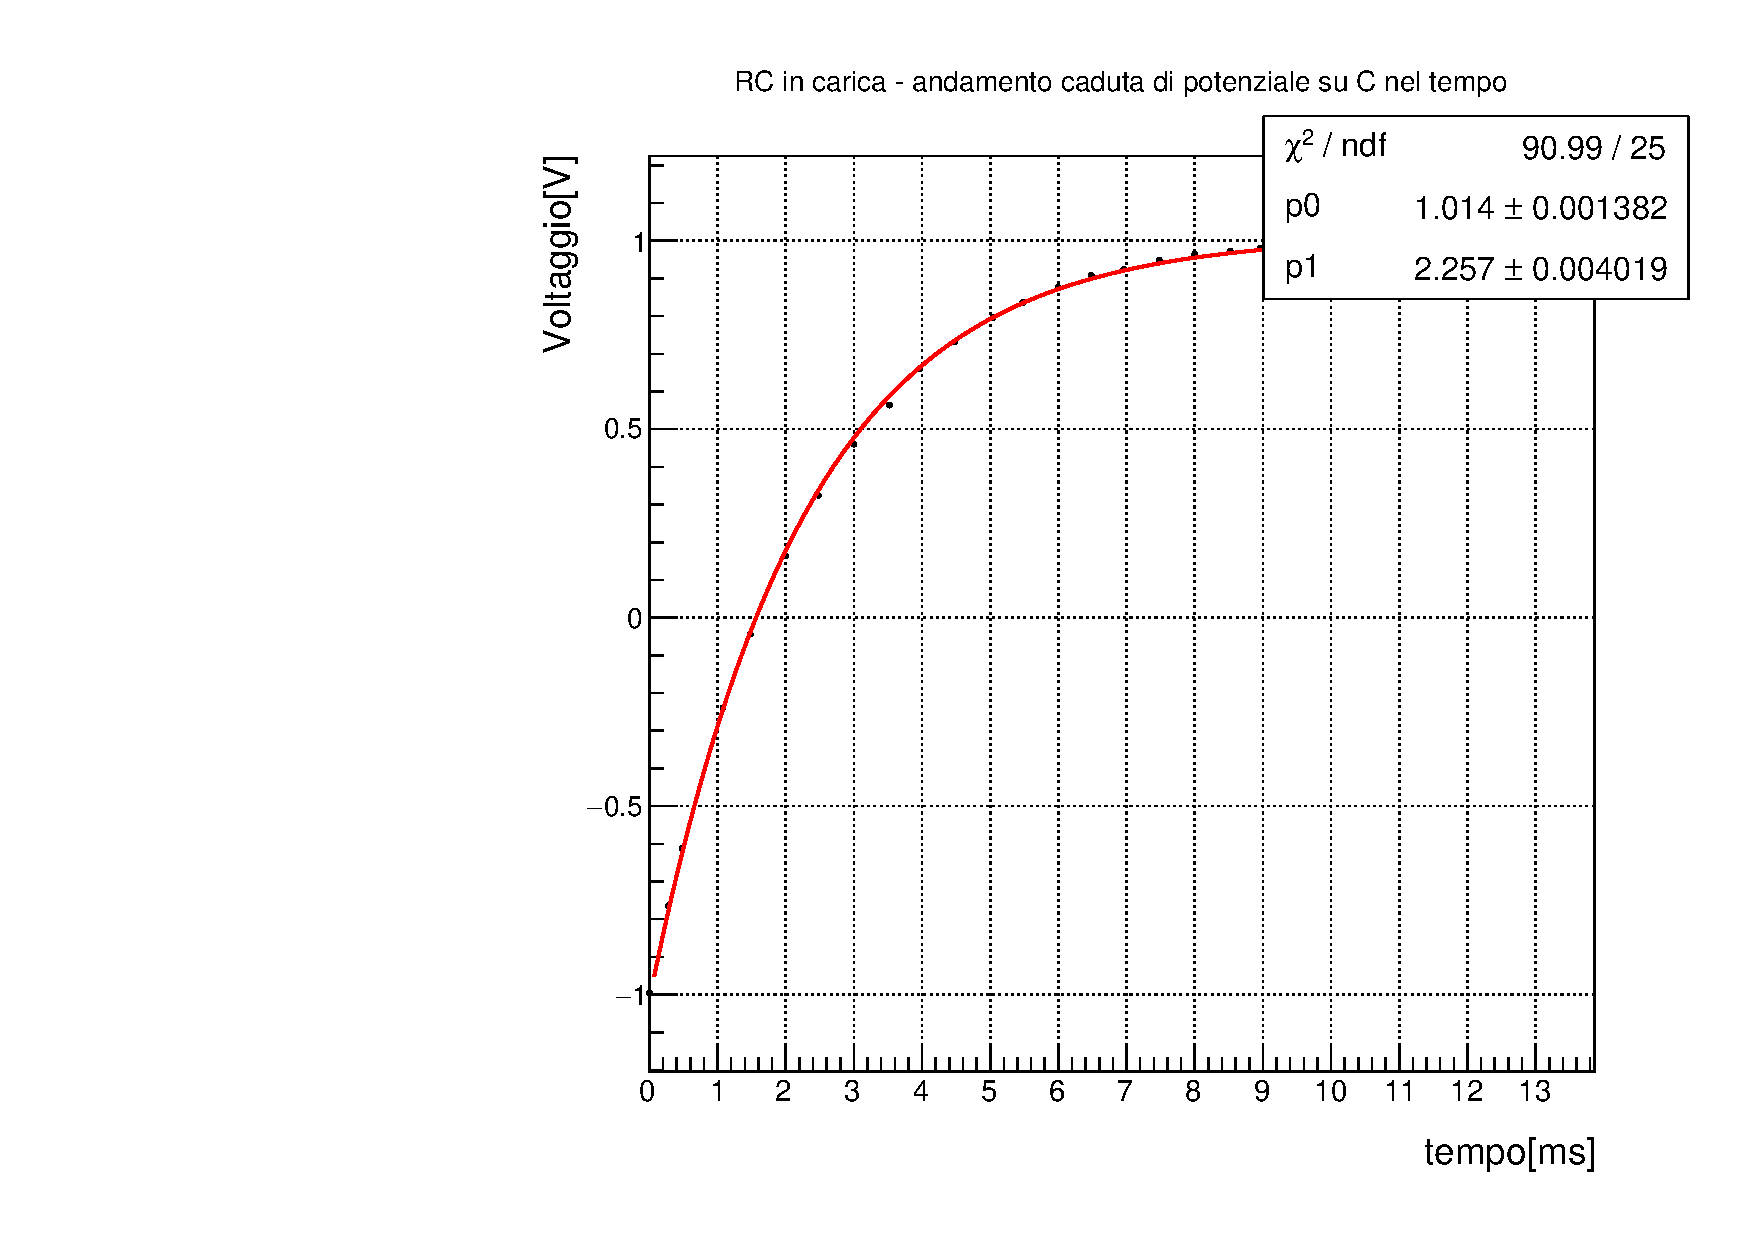
\includegraphics{prima parte/crescitaRC.pdf}
		} %close resize
	} %close centering
	\caption{funzione usata per l'interpolazione:  \(p_{0} (1 - 2e^{\frac{-x}{p_{1}}} )\)}

    \label{fig:RC_su_C}

\end{figure}

\noindent Osserviamo una certa discrepanza tra il valore del \(\chi^{2} = 178.3\) (ricavato dal programma ROOT di CERN) e il numero dei gradi di libertà Ndf = 25. Siccome l'andamento funzionale atteso sembra essere stato rispettato dai dati, associamo questa problematica ad una stima degli errori sul voltaggio scarsamente realistica, utilizzando quindi il risultato del test stimiamo \(\sigma_{V}\) a posteriori come \(\sigma_{V} \cdot \frac{\chi^{2}}{Ndf} = \sigma_{V} \cdot 7\) che in media corrisponde a circa 0.03 V di errore su ogni misura effettuata. \\

\noindent Eseguendo nuovamente l'interpolazione dopo aver corretto le incertezze otteniamo dei parametri con errori più veritieri: \\


 \(p_{0} = V_{0} = 1.014 \pm 0.007 V \)  da confrontare con il valore indicato sul generatore: 1.00 \(\pm\) 0.01 V\(\rightarrow \) t = 1.1, PValue = 27\%;\\
 
 \(p_{1} = \tau_{RC} = 2.26 \pm 0.02 \) ms è il tempo caratteristico del sistema, quantifica la tempistica necessaria per completare la carica del nostro condensatore; da tale dato, conoscendo R = 0.989\(\pm\) 0.001 k\(\Omega\) è possibile ricavare una stima della capacità C:
 
\[\hat{C} = \frac{\tau}{R}=  \frac{2.26ms}{0.989 k\Omega} = 2.28169 \mu F \hspace{1cm} \sigma_{\hat{C}} = \sqrt{\left(\frac{\sigma_{\tau}}{R}\right)^{2} + \left(\frac{\tau \sigma_{R}}{R^{2}}\right)^{2}} = 0.020451 \mu F\] 

\noindent Dunque una prima stima per C risulta \(\hat{C} =  2.28 \pm 0.02 \mu F\), da un confronto con il valore atteso \(C_{att} = 2.42 \pm 0.01 \mu\)F tramite il test t-Student risulta:
\[t = \frac{\left| C_{att} - \hat{C}\right|}{\sqrt{\sigma^{2}_{C_{att}} + \sigma_{\hat{C}}}} = 6 \rightarrow PValue = NA\]

La probabilità che la nostra stima si distribuisca con andamento gaussiano attorno al valore supposto come valore vero è prossima allo 0\(\%\), avanziamo dunque due ipotesi: il valore vero non corrisponde a quello indicato dal multimetro, oppure degli errori non casuali ma di tipo sistematico sono subentrati durante lo svolgimento dell'esperimento. Procediamo con l'analisi del secondo set di dati per approfondire la questione. \\

\noindent I dati relativi alla ddp su R sono riportati nel grafico in Figura \ref{fig:RC_su_R}, completo di interpolazione eseguita seguendo il modello teorico
\[V_{R}(t) = 2 \cdot V_{0} e^{\frac{t}{\tau}}\]

che si ottiene applicando le leggi di Kirchoff al circuito CR esplicitando la corrente I(t) (ricordiamo che \(V_{R}(t) = I(t) \cdot R\)). \\

\begin{figure}[!htbp]

	\makebox[1 \textwidth][c]{       %centering table
		\resizebox{0.68 \textwidth}{!}{   %resize table
			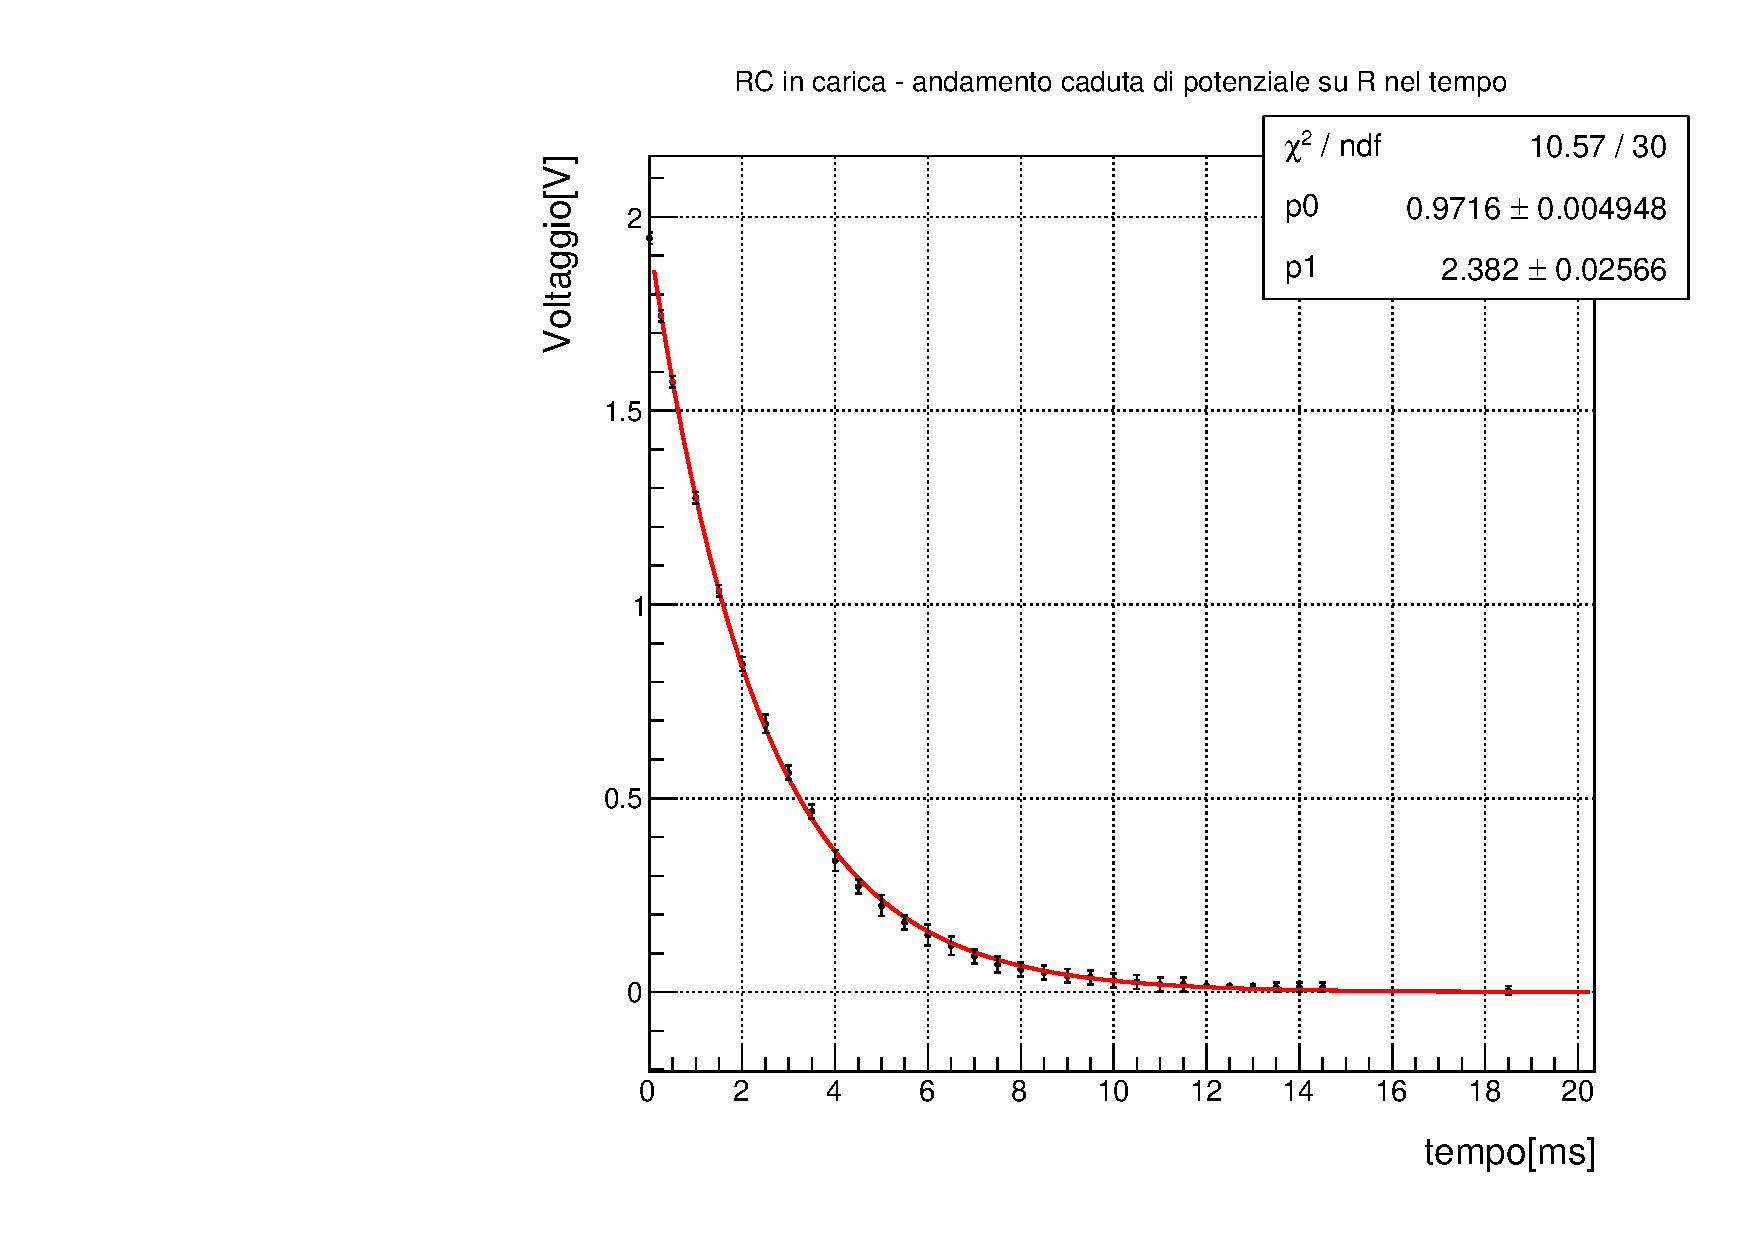
\includegraphics{prima parte/decrescitaRC.pdf}
		} %close resize
	} %close centering
	\caption{funzione usata per l'interpolazione:  \(2p_{0}e^{\frac{-x}{p_{1}}}\) }

    \label{fig:RC_su_R}

\end{figure}

\noindent Notiamo che anche in questo caso il chi quadro è 3 volte maggiore del suo valore di aspettazione Ndf = 30, perciò prima di cimentarci nei calcoli abbiamo scalato tutte le incertezze \(\sigma_{V}\) di un fattore 3, per poi ottenere i seguenti risultati: \\

\( p_{0} = V_{0} =  0.972 \pm 0.005\)V  da confrontare sempre con il valore impostato inizialmente: 1.00 pm 0.01 V \(\rightarrow\) t = 2, PValue = 5\%; \\

\(  p_{1} =  \tau_{RC} =   2.38 \pm 0.03\)ms da cui abbiamo calcolato nuovamente C: \\
\[\hat{C} = \frac{2.38ms}{0.989 k\Omega} =  2.40816  \mu F \hspace{1cm} \sigma_{\hat{C}} = \sqrt{\left(\frac{\sigma_{\tau}}{R}\right)^{2} + \left(\frac{\sigma_{R}\tau}{R^{2}} \right)^{2}} = 0.0260623 \mu F\]

\noindent Perciò la seconda stima di C è \(\hat{C} =  2.41 \pm 0.03 \mu F\), confrontandola tramite il test t-Student con il valore atteso \(C_{att} = 2.42 \pm 0.01 \mu\)F ottenuto con il multimetro otteniamo:

\[t = \frac{\left| C_{att} - \hat{C}\right|}{\sqrt{\sigma^{2}_{C_{att}} + \sigma_{\hat{C}}}} = 0.3 \rightarrow PValue = 76.42\%\]

\noindent Data l'evidente concordanza tra la seconda stima per C ed il suo valore misurato direttamente con il multimetro, supponiamo di aver incontrato dei fattori di disturbo che hanno alterato svolgimento del primo esperimento. 

\pagebreak

\subsection{Circuito RL}
\label{sec:circuitoRL}

Per il circuito RL abbiamo adoperato la medesima resistenza R = \(0.989 \pm 0.001 k\Omega\) e una induttanza il cui valore è da determinare tramite l'analisi delle misure effettuate. \\
Il circuito costruito per la misura ai capi di L è un RL, come mostrato in figura; la misura della ddp ai capi di R è stata eseguita ancora una volta scambiando i due componenti. \\


\begin{figure}[!ht]

	\makebox[1 \textwidth][c]{       %centering table
		\resizebox{0.7 \textwidth}{!}{   %resize table
			\includegraphics{prima parte/schemaRL.png}
		} %close resize
	} %close centering
	\caption{schema di un circuito RL}

    \label{fig:RL_schema}

\end{figure}

\noindent Affianco al componente L nello schema abbiamo aggiunto la resistenza parassita dovuta all'induttanza, solitamente dell'ordine di qualche \(\Omega\), che potrebbe influire nelle misure ottenute quando ancora \(f\) è particolarmente alta, ovvero negli istanti dove comincia un picco dell'onda quadra. \\

\subsubsection*{Dati raccolti}
Abbiamo proceduto analogamente alla raccolta dati relativa al circuito RC, campionando solo i grafici che corrispondono al fenomeno di carica dell'induttore. \\
Si osservi che questa volta l'errore strumentale sui tempi varia da 0.02 \(\mu\)s a 2\(\mu\)s seconda dell'ordine di grandezza della misura, mentre l'errore strumentale sul voltaggio è sempre 2mV. 


\begin{table}[!htbp]
    \captionsetup{labelformat=empty}
    \caption{Tabella2: circuiti RL e LR in carica}
    
    \resizebox{13cm}{!}{

    \begin{minipage}{.5\linewidth}
      \caption{(a) ddp ai capi di L}
      \centering
       \begin{tabular}{c|cc|c}

        t[\(\mu\)s] & V & [mV] & \(V_{medio}\)[V] \\
        \hline
        \hline
        
        5.00 & 1760 &1800 & 1.78 \(\pm\) 0.02\\
        \hline
        10.0 & 1600& 1580 & 1.59 \(\pm\) 0.01\\
        \hline
        15.0 & 1440 &1420 & 1.43 \(\pm\) 0.01\\
        \hline
        20.0 & 1280 &1300 & 1.29 \(\pm\) 0.01\\
        \hline
        25.0 & 1140& 1180 & 1.16 \(\pm\) 0.02\\
        \hline
        30.0 & 1040& 1060 & 1.05 \(\pm\) 0.01\\
        \hline
        35.0 & 960 &920 & 0.94 \(\pm\) 0.02\\
        \hline
        40.0 & 840 &820 & 0.83 \(\pm\) 0.01\\
        \hline
        45.0 & 760 &740 & 0.75 \(\pm\) 0.01\\
        \hline
        50.0 & 680 &700 & 0.69 \(\pm\) 0.01\\
        \hline
        55.0 & 620 &640 & 0.63 \(\pm\) 0.01\\
        \hline
        60.0 & 560 &540 & 0.55 \(\pm\) 0.01\\
        \hline
        65.0 & 480 &520 & 0.50 \(\pm\) 0.02\\
        \hline
        70.0 & 480 &440 & 0.46 \(\pm\) 0.02\\
        \hline
        75.0 & 400 &420 & 0.41 \(\pm\) 0.01\\
        \hline
        80.0 & 380 &360 & 0.37 \(\pm\) 0.01\\
        \hline
        85.0 & 360 &320 & 0.34 \(\pm\) 0.02\\
        \hline
        90.0 & 300 &320 & 0.31 \(\pm\) 0.01\\
        \hline
        95.0 & 300 &260 & 0.28 \(\pm\) 0.02\\
        \hline
        100.0 & 290& 270 & 0.28 \(\pm\) 0.01\\
        \hline
        105.0 & 200& 220 & 0.21 \(\pm\) 0.01\\
        \hline
        110.0 & 240& 220 & 0.23 \(\pm\) 0.01\\
        \hline
        115.0 & 200 &180 & 0.19 \(\pm\) 0.01\\
        \hline
        120.0 & 180 &160 & 0.17 \(\pm\) 0.01\\
        \hline
        125.0 & 160 &140 & 0.15 \(\pm\) 0.01\\
        \hline
        130.0 & 140 &120 & 0.13 \(\pm\) 0.01\\
        \hline
        135.0 & 120 &100 & 0.11 \(\pm\) 0.01\\
        \hline
        140.0 & 120 &100 & 0.11 \(\pm\) 0.01\\
        \hline
        145.0 & 100 &80 & 0.09 \(\pm\) 0.01\\
        \hline 
        150.0 & 80& 60 & 0.07 \(\pm\) 0.01\\
        \hline
        155.0 & 80& 100 & 0.09 \(\pm\) 0.01\\
        \hline
        160.0 & 80& 70 & 0.075 \(\pm\) 0.005\\
        \hline
        165.0 & 50 &70 & 0.06 \(\pm\) 0.01\\
        \hline
        170.0 & 70 &50 & 0.06 \(\pm\) 0.01\\
        \hline
        175.0 & 50 &50 & 0.05 \(\pm\) 0.002\\
        \hline
        180.0 & 50& 30 & 0.04 \(\pm\) 0.01\\
        \hline
        185.0 & 20& 50 & 0.035 \(\pm\) 0.015\\
       \hline
       \hline
    \end{tabular}
    \end{minipage}%
    \begin{minipage}{.7\linewidth}
      \centering
         \captionsetup{labelformat=empty}
    	 \caption{(b) ddp ai capi di R}
            \begin{tabular}{c|cc|c}

        t[\(\mu\)s] & V & [mV] & \(V_{medio}\)[V] \\
        \hline
        \hline
        0.00& -794& -810& -0.802 \(\pm\)  0.008\\
        \hline
        6.00& -676& -684& -0.680  \(\pm\) 0.004\\
        \hline
        10.0& -548& -498&  -0.523  \(\pm\) 0.025\\
        \hline
        16.0& -362& -348 & -0.355 \(\pm\)  0.007\\
        \hline
        20.0& -252& -228 & -0.240 \(\pm\)  0.012\\
        \hline
        26.0& -100& -80 & -0.09  \(\pm\) 0.01\\
        \hline
        30.0& -20& 2 &  -0.009  \(\pm\) 0.011\\
        \hline
        36.0& 104& 118 & 0.111  \(\pm\) 0.007\\
        \hline
        40.0& 184& 164 & 0.174  \(\pm\) 0.01\\
        \hline
        46.0& 276& 260 & 0.268 \(\pm\)  0.008 \\
        \hline
        50.0& 324& 340 &  0.332  \(\pm\) 0.008 \\
        \hline
        56.0& 412& 396 &  0.404  \(\pm\) 0.008\\
        \hline
        60.0& 444&460 & 0.452 \(\pm\)  0.008\\
        \hline
        66.0& 516& 500 & 0.508 \(\pm\)  0.008\\
        \hline
        70.0& 556& 538 &  0.547 \(\pm\)  0.009\\
        \hline
        76.0& 588& 612  & 0.6 \(\pm\)  0.012\\
        \hline
        80.0&620& 634 & 0.627 \(\pm\)  0.007\\
        \hline
        86.0& 628& 644 &0.636 \(\pm\)  0.008\\
        \hline
        90.0& 644& 668  & 0.656 \(\pm\) \(\pm\)  0.012\\
        \hline
        96.0&  692 & 676  &  0.684 \(\pm\)  0.008\\
        \hline
        100&  708&724  & 0.716  \(\pm\) 0.008\\
        \hline
        106& 732&748 &  0.74 \(\pm\)  0.008\\
        \hline
        110& 750& 764  &  0.757 \(\pm\)  0.007\\
        \hline
        116& 756& 772  &  0.764 \(\pm\)  0.008\\
        \hline
        120& 774& 784 &  0.779  \(\pm\) 0.005\\
        \hline
        126& 804& 776  &  0.79 \(\pm\)  0.01\\
        \hline
        130& 804& 788  & 0.796 \(\pm\)  0.008\\
        \hline
        136& 804& 820  & 0.812 \(\pm\)  0.008\\
        \hline
        140& 820& 836  &0.828 \(\pm\)  0.008\\
        \hline
        146& 818& 834 & 0.826 \(\pm\)  0.008\\
        \hline
        150& 834& 838  & 0.836  \(\pm\) 0.002\\
        \hline
        156& 834& 848  &  0.841  \(\pm\) 0.007\\
        \hline
        160&  846& 860  &  0.847 \(\pm\)  0.007\\
        \hline
        168& 864&842 & 0.853  \(\pm\) 0.007\\
        \hline
        176& 854& 840  & 0.853  \(\pm\) 0.011\\
        \hline
        180& 870& 852 & 0.861 \(\pm\)  0.009\\
        \hline
        186& 870& 856  & 0.863  \(\pm\) 0.007\\
        \hline
        190& 880& 856  & 0.868  \(\pm\) 0.012\\
        \hline
        196&  864& 876 & 0.87 \(\pm\)  0.006\\
        \hline
        206& 868&882 &  0.875 \(\pm\)  0.007\\
        \hline
        210& 868& 892  & 0.88 \(\pm\)  0.012\\
        \hline
        216& 892& 868 & 0.88 \(\pm\)  0.012\\
        \hline
        220& 868& 882 & 0.875 \(\pm\)  0.007\\
        \hline
        226& 868& 886 & 0.877 \(\pm\) 0.009\\
        \hline
        230& 880& 892 & 0.886 \(\pm\)  0.006\\
        \hline
        \hline
    \end{tabular}
    \end{minipage} 
    }
    \caption{dove \(\sigma_{V} = 0 V\) abbiamo usato l'incertezza dello strumento = 0.002 V}

\end{table}


\pagebreak

\subsubsection*{Analisi dati e commenti}
\label{subsec:res_parassite}
Eseguendo l'interpolazione dei dati in Tabella 2 (a) con la formula attesa per \(V_{L}\) nell'ipotesi T\(\gg \tau\) poichè T\(\approx 0.1\)s e \(\tau = \frac{L}{R} \approx 10^{-6}s\) :
\[V_{L}(t) = 2V_{0}e^{-\frac{t}{\tau}}\]
otteniamo il seguente grafico. \\

\begin{figure}[!ht]

	\makebox[1 \textwidth][c]{       %centering table
		\resizebox{0.80 \textwidth}{!}{   %resize table
			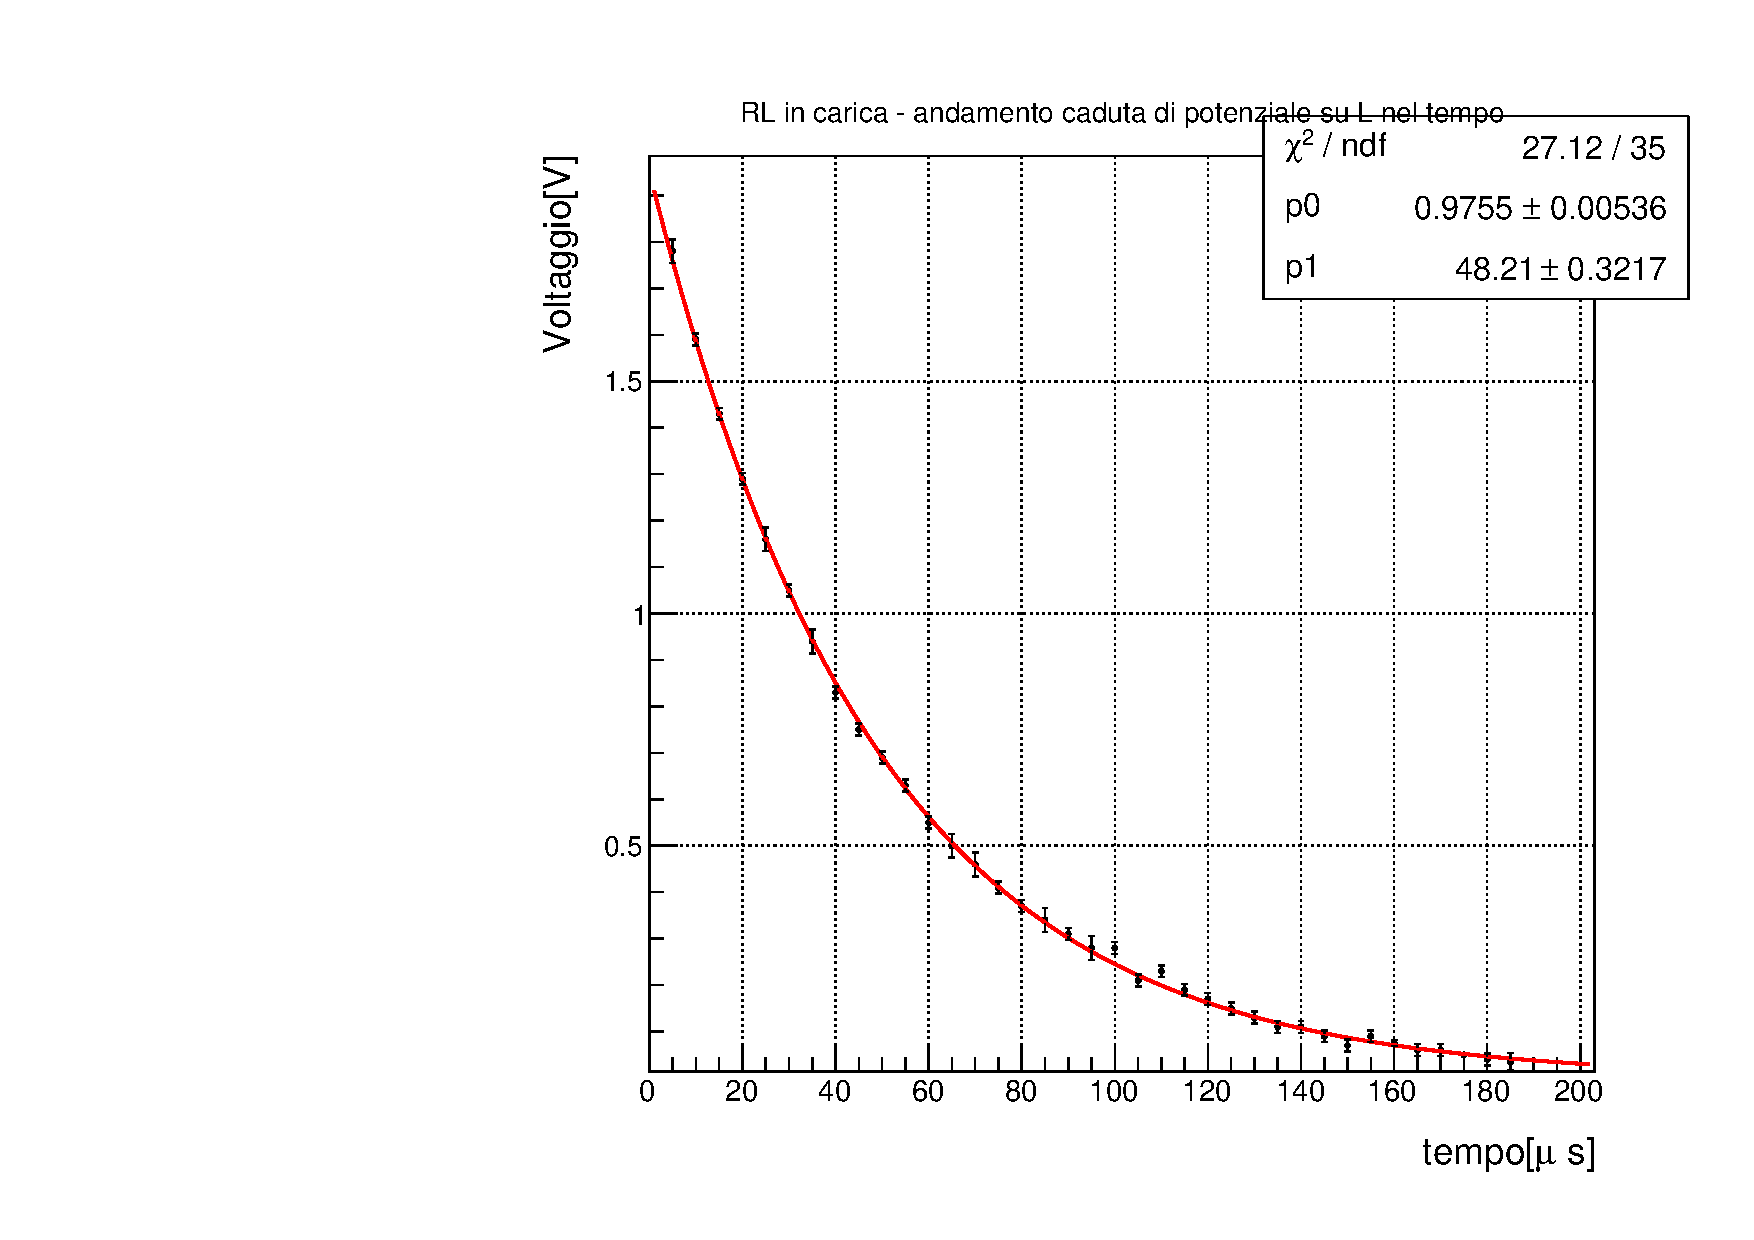
\includegraphics{prima parte/decrescitaRL.pdf}
		} %close resize
	} %close centering
	\caption{funzione usata per l'interpolazione:  \(2p_{0}e^{\frac{-x}{p_{1}}}\) }

    \label{fig:RL_su_L}

\end{figure}
\noindent Per prima cosa osserviamo che la risposta del circuito RL ad un aumento repentino di tensione come quello che avviene per t = 0 richiede qualche istante in più rispetto al caso con C; abbiamo infatti cominciato a campionare il grafico di \(V_{L}\) a partire da 5\(\mu\)s poichè in 0s l'oscilloscopio riportava ancora un valore negativo. L'induttore infatti è tipicamente un componente che tende ad opporsi alla variazione di corrente nel circuito, e la sua resistenza parassita è massima all'inizio del fenomeno, dove notiamo che \(V_{L}\) non raggiunge il massimo potenziale ma si ferma 1.78V \(<\) dei 2V attesi nel caso ideale. \\

\noindent Osserviamo inoltre che il test del chi quadro riporta un valore di \(\chi^{2} = 43.52\), di poco superiore a Ndf = 34. Probabilmente le incertezze relative al voltaggio sono state sottostimate di un fattore \(\frac{\chi^{2}}{Ndf} = 1.28\), quindi abbiamo eseguito nuovamente la ricerca dei parametri moltiplicando ogni \(\sigma_{y}\) per 1.28. \\

\noindent I parametri risultati dall'analisi eseguita con ROOT sono:\\

\(  p0 = V_{g} = 0.976 \pm   0.005 V  \), da confrontare con \(1.000\pm 0.001\)V impostato sul generatore \(\rightarrow t = 5, PValue = NA\), il fatto che questo PValue non sia accettabile è probabilmente dovuto alla resistenza parassita di L; \\

\(  p1 = \tau_{RL}= 48.2 \pm 0.3  \mu\)s, da cui è possibile ricavare una stima di L conoscendo R come \(R = 0.989\pm 0.001 k\Omega\). Esprimendo \(\tau\) in \(\mu s\) e R in \(M \Omega\) si ottiene:

\[\hat{L} = \tau_{RL}\cdot R = 0.0477 H \] \[\sigma_{L}= \sqrt{(\sigma_{\tau} R)^{2} + (\sigma_{R}\tau_{RL})^{2}} = 0.0003 H\] 

\noindent dunque \(\hat{L} = 47.7 \pm 0.3 \), mH che possiamo confrontare con la stima ottenuta dal secondo grafico.\\

\noindent Il voltaggio ai capi della resistenza R segue, secondo le leggi di Kirchoff, il seguente andamento temporale:
\[V_{R}(t) = I(t)\cdot R = V_{0}\left(1 - 2\cdot e^{-\frac{t}{\tau}}\right)\]
l'interpolazione eseguita corrisponde al grafico in Figura \ref{fig:RL_su_R}, notiamo che il limite asintotico del nostro grafico non tende a 1V= \(V_{0}\) ma a 0.8V. \\

\begin{figure}[!ht]

	\makebox[1 \textwidth][c]{       %centering table
		\resizebox{0.90 \textwidth}{!}{   %resize table
			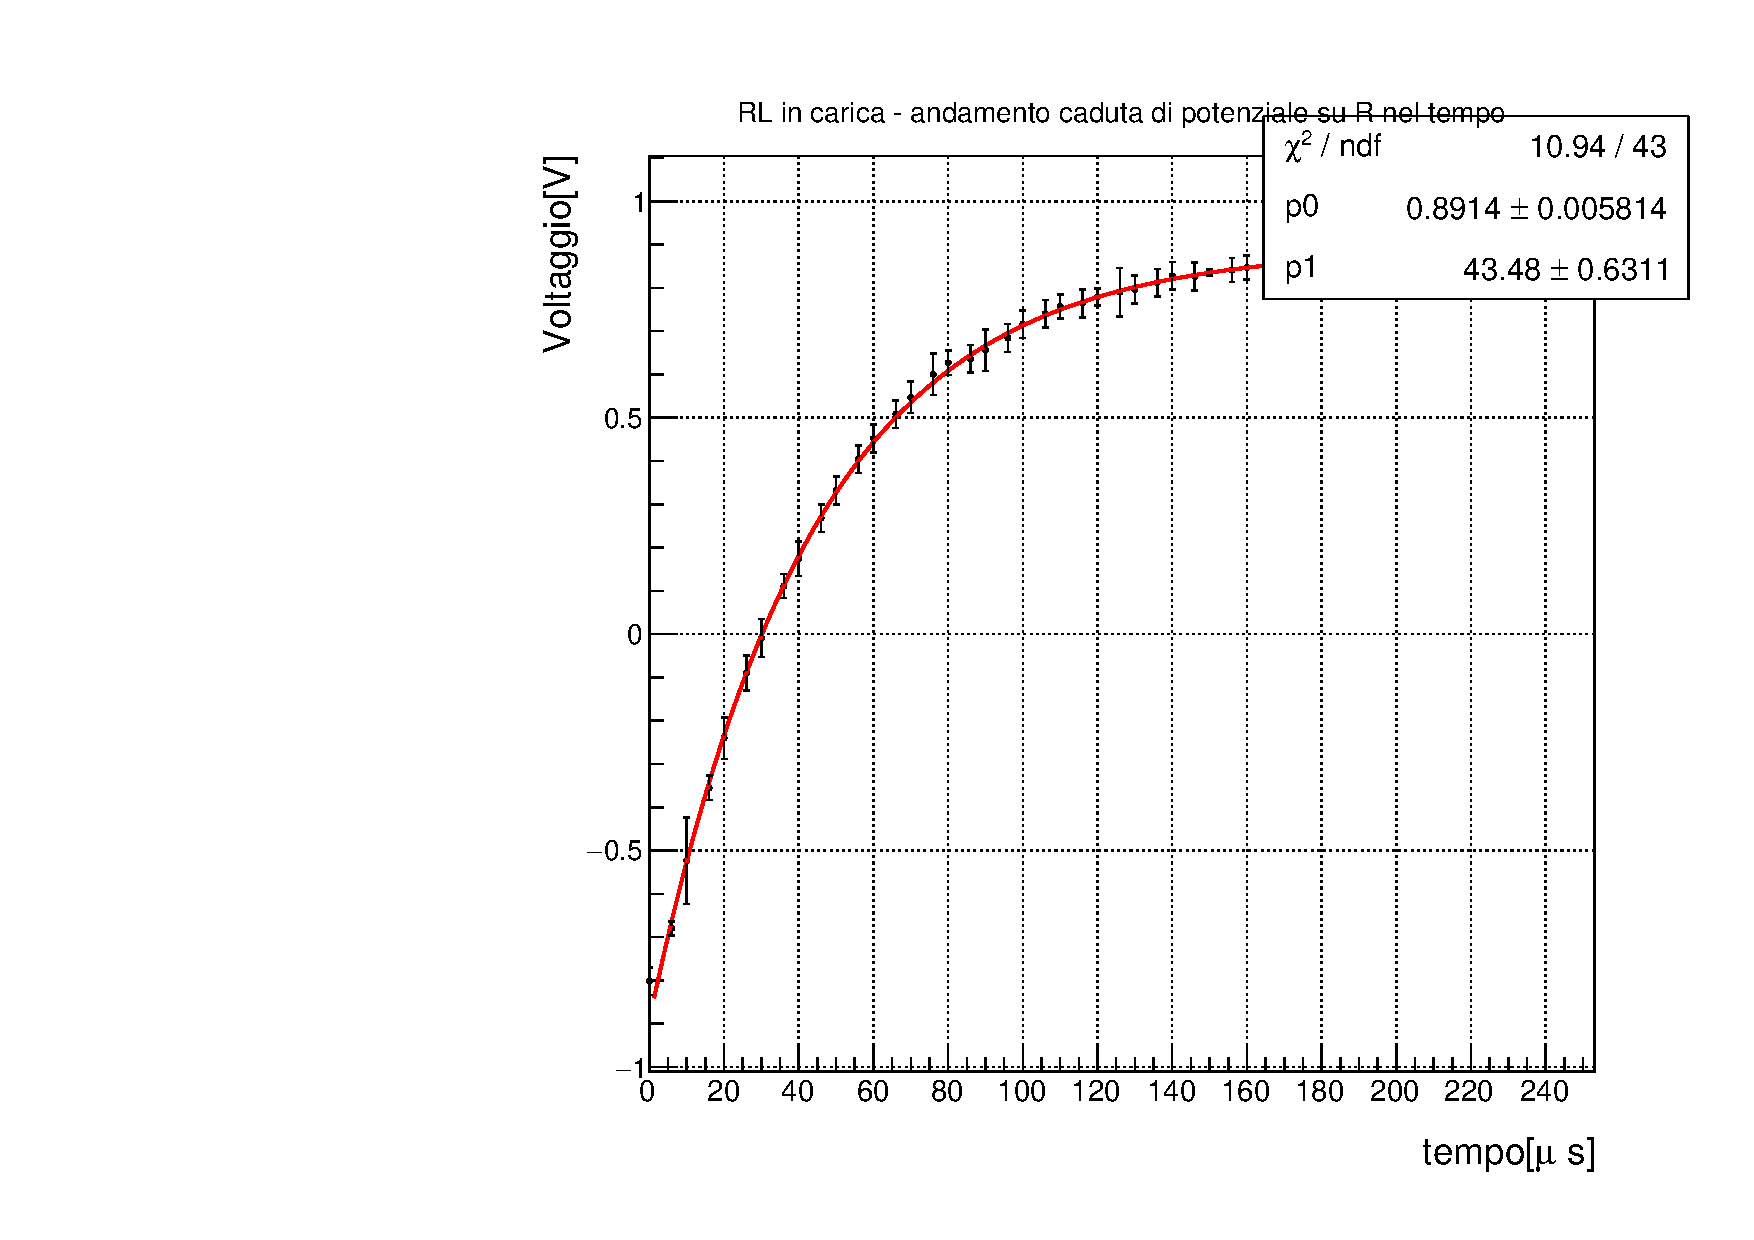
\includegraphics{prima parte/crescitaRL.pdf}
		} %close resize
	} %close centering
	\caption{funzione usata per l'interpolazione:  \(p_{0}( 1 - 2e^{\frac{-x}{p_{1}}})\) }

    \label{fig:RL_su_R}

\end{figure}
\noindent Per comprendere il motivo di questa rappresentazione inaspettata del grafico, che parte da -0.80V e arriva ad un massimo di 0.89V, facciamo riferimento allo schema circuitale di un partitore di tensione. Avanziamo quindi l'ipotesi che la nostra resistenza di carico R non sia l'unica ad avere un valore considerevole, ma che siano presenti delle resistenze parassite \(R_{par}\), dovute ad esempio a generatore e induttore, altrettanto notevoli. Attenzione, la \(R_{par}\) dovuta all'induttanza gioca un ruolo importante nel partitore solo all'avvio della carica, al tempo\\ t = 0, dove la frequenza è particolarmente alta. Questo spiega la differenza dei valori misurati in partenza e in arrivo, che nel caso ideale dovrebbero essere uguali. \\
Nel caso del partitore si tensione, la misura del potenziale ai capi di un componente (R) dipende dalla ripartizione della tensione di tutti i componenti che avviene in base ai loro valori relativi; quindi \(V_{R, reale}(t) = \frac{V_{R, ideale}(t) \cdot R}{R_{par} + R}\). \\

\noindent Notiamo inoltre che il risultato del test del chi quadro mostra una certa discordanza tra misure e modello atteso, siccome l'andamento funzionale ipotizzato rimane valido, supponiamo che la discordanza sia dovuta ad incertezze stimate per difetto rispetto a quelle reali. \\

\noindent È nostro interesse effettuare una stima delle resistenze parassite che hanno influito sulla misura, guardiamo per esempio il regime asintotico, dove \(R_{par}\) dovuta a L \(\approx 0\), e stimiamo il coefficiente \(\alpha\) di cui il voltaggio è stato attenuato prendendo in considerazione l'ultimo punto della nostra tabella; la sicurezza con cui conosciamo questo fattore dipende dalla precisione della misura effettuata, che abbiamo riscalato di \(\frac{\chi^{2}}{Ndf} = 4\).

\[\alpha = \frac{R}{R + R_{par}} = \frac{V_{real}}{V_{0}} = \frac{0.886V}{1V} \pm 0.03 \]

da cui, considerando \(\sigma_{R} = 1 \Omega\) e \(\sigma_{\alpha} = 0.03\), otteniamo che \\
\[R_{par} = R\cdot \frac{1 - \alpha}{\alpha} = 127.3 \pm 30 \Omega\]

\noindent Ora osserviamo i risultati dell'interpolazione tenendo in considerazione le resistenze parassite stimate. I parametri ottenuti dal fit sono \(p0 = V_{0} = 0.891 \pm  0.001 \)V, e \( p1 =\tau_{RL} = 43.5 \pm 0.2 \mu s\) da cui calcoliamo di nuovo L considerando questa volta che la resistenza equivalente del circuito è \(R_{par} + R = 1.116 \pm 0.03 k\Omega\), nei calcoli abbiamo espresso \(R_{eq}\) in M\(\Omega\)\\

\[\hat{L} = \tau_{RL}\cdot (R + R_{par}) = 0.049 H\]
\[ \sigma_{L}= \sqrt{(\sigma_{\tau} (R + R_{par}) \cdot10^{-3})^{2} + (\sigma_{Req} \cdot 10^{-3}\tau_{RL})^{2}} = 0.001 H\] 

\noindent perciò \(\hat{L} = 49 \pm 1\) mH da confrontare con quella precedentemente ottenuta tramite il test t-Student:

\[t = \frac{\left|L_{1} - L_{2} \right|}{\sqrt{\sigma^{2}_{L1} + \sigma^{2}_{L2}} } = 1.2 \rightarrow PValue = 23.01\% \]

\pagebreak

\section{Parte seconda}

Nella seconda parte dell'esperienza abbiamo studiato il comportarmento di un circuito RCL nei regimi sottosmorzato, sovrasmorzato e di smorzamento critico.

\subsection{Obiettivi e metodo adottato}
Questa parte dell'esperienza richiedeva di selezionare diverse resistenze a seconda del regime d'interesse, abbiamo perciò utilizzato la scatola delle resistenze variabili e selezionato in totale 3 diversi valori per R. Lo schema e la realizzazione del circuito sono rappresentati in Figura \ref{fig:RLC}. \\

\noindent L'obiettivo era ancora una volta di verificare il modello per I(t) dedotto dalle leggi di Kirchoff applicate al circuito, quando quest'ultimo è sottoposto ad una tensione impulsata. Il procedimento adottato consiste dunque nel rilevare l'andamento temporale del voltaggio ai capi di R nei 3 regimi, il quale è proporzionale, come ben sappiamo, alla corrente.


\begin{figure}[!h]
\hfill
\subfigure[schema di un circuito LCR]{\includegraphics[width=6cm]{seconda parte/schemaRCL.png}}
\hfill
\subfigure[realizzazione in laboratorio]{\includegraphics[width=5cm]{seconda parte/RLC_foto.png}}
\hfill
\caption{ }
\label{fig:RLC}
\end{figure}



\subsection{regime sottosmorzato}
\label{subsec:sottosmorzamento}

Dal momento che, eseguendo una media pesata tra \(L_{1}\) ed \(L_{2}\), la nostra stima per L risulta \(\hat{L} = 47.80734 \pm 8 \cdot 10^{-5} \) mH e che il nuovo condensatore ha C = 99\(\pm 1\) nF, il circuito avrà un comportamento sottosmorzato per \(R < \sqrt{\frac{4 \cdot L}{C}} = 1.390 k\Omega \)

\subsubsection*{Dati raccolti}
La misura della capacità C = 99\( \pm 1\) nF è stata effettuata con il multimetro palmare. La scelta di cambiare condensatore è stata dettata dal fatto che una capacità dell'ordine dei \(\mu F\) risultava eccessiva; abbiamo infatti osservato una distorsione del grafico V(t) in sottosmorzamento, che era più simile all'andamento tipico del sovrasmorzamento.  L'accumulo di elevata energia da parte del condensatore stava accentuando l'effetto delle resistenze interne dei componenti del circuito, disturbando il fenomeno ricercato in origine. \\
Dopo aver trovato il condensatore adatto ai nostri scopi, abbiamo scelto una resistenza pari a R = 101.6\(\pm 0.1 \Omega\) dalla scatola delle resistenze variabili (misurazione effettuata con il multimetro palmare) e infine ricavato le misure per il voltaggio ai capi di R per ogni istante selezionato.

\begin{table}[!htbp]
\centering
    \captionsetup{labelformat=empty}
    	 \caption{Tabella3: circuito LCR - regime sottosmorzato}
    \resizebox{8cm}{!}{

    \begin{tabular}{c|cc|c}

        t[\(\mu\)s] & V & [mV] & \(V_{medio}\)[V] \\
        \hline
        \hline
        0& 4.00& 8.00& 0.006 \(\pm\) 0.002\\
        \hline
        42& 152& 156& 0.154 \(\pm\)  0.002\\
        \hline
        76& 216& 220& 0.218 \(\pm\)  0.002\\
        \hline
        98& 232& 236&  0.234 \(\pm\)  0.002\\
        \hline
        126& 226& 220& 0.223 \(\pm\)  0.003\\
        \hline
        154& 172& 176& 0.174 \(\pm\)  0.002\\
        \hline
        186& 90.0& 84.0&  0.087 \(\pm\)  0.003\\
        \hline
        259& -84.0& -88.0& -0.086 \(\pm\)  0.002\\
        \hline
        330& -132&-136& -0.134\(\pm\)   0.002\\
        \hline
        382& -88.0& -92.0&  -0.09  \(\pm\) 0.002\\
        \hline
        448&20.0& 24.0& 0.022 \(\pm\)  0.002\\
        \hline
        535& 92& 88.0& 0.09 \(\pm\)  0.002\\
        \hline
        607& 52.0& 56.0& 0.054  \(\pm\) 0.002\\
        \hline
        666& -8.00& -4.00& -0.006 \(\pm\)  0.002\\
        \hline
        708& -40.0& -37.0& -0.0385 \(\pm\)  0.0015\\
        \hline
        775& -52.0& -48.0&  -0.05 \(\pm\)  0.002\\
        \hline
        842& -16.0& -13.0&  -0.0145 \(\pm\)  0.0015\\
        \hline
        912& 28.0& 24.0&  0.026 \(\pm\)  0.002\\
        \hline
        953& 36.0& 40.0&0.038 \(\pm\)  0.002\\
        \hline
        1010& 32.0& 28.0& 0.03\(\pm\)   0.002\\
        \hline
        1060& 16.0& 14.0&0.015\(\pm\)   0.001\\
        \hline
        1130& -12.0& -8.00&  -0.01\(\pm\)   0.002\\
        \hline
        1210& -16.0& -20.0&  -0.018 \(\pm\)  0.002\\
        \hline
        1270& -8.00& -4.00& -0.006  \(\pm\) 0.002\\
        \hline
        1320& 8.00&4.00& 0.006\(\pm\)   0.002\\
        \hline
        1400& 8.00& 12.00& 0.01 \(\pm\)  0.002\\
        \hline
        1470& 8.00& 4.00&0.006 \(\pm\)  0.002\\
        \hline
    \end{tabular}
    }
\caption{errore strumentale: sui tempi = 2 \(\mu s\) e sul voltaggio = 2mV}
\end{table}


\subsubsection*{Analisi dati e commenti}
L'interpolazione eseguita a partire dal modello atteso per I(t), ovvero
\[I(t) = Ae^{-\gamma t}sin(\beta t)\]
sui dati riportati in Tabella3 ha prodotto il seguente risultato \\

\begin{figure}[!ht]

	\makebox[1 \textwidth][c]{       %centering table
		\resizebox{0.80 \textwidth}{!}{   %resize table
			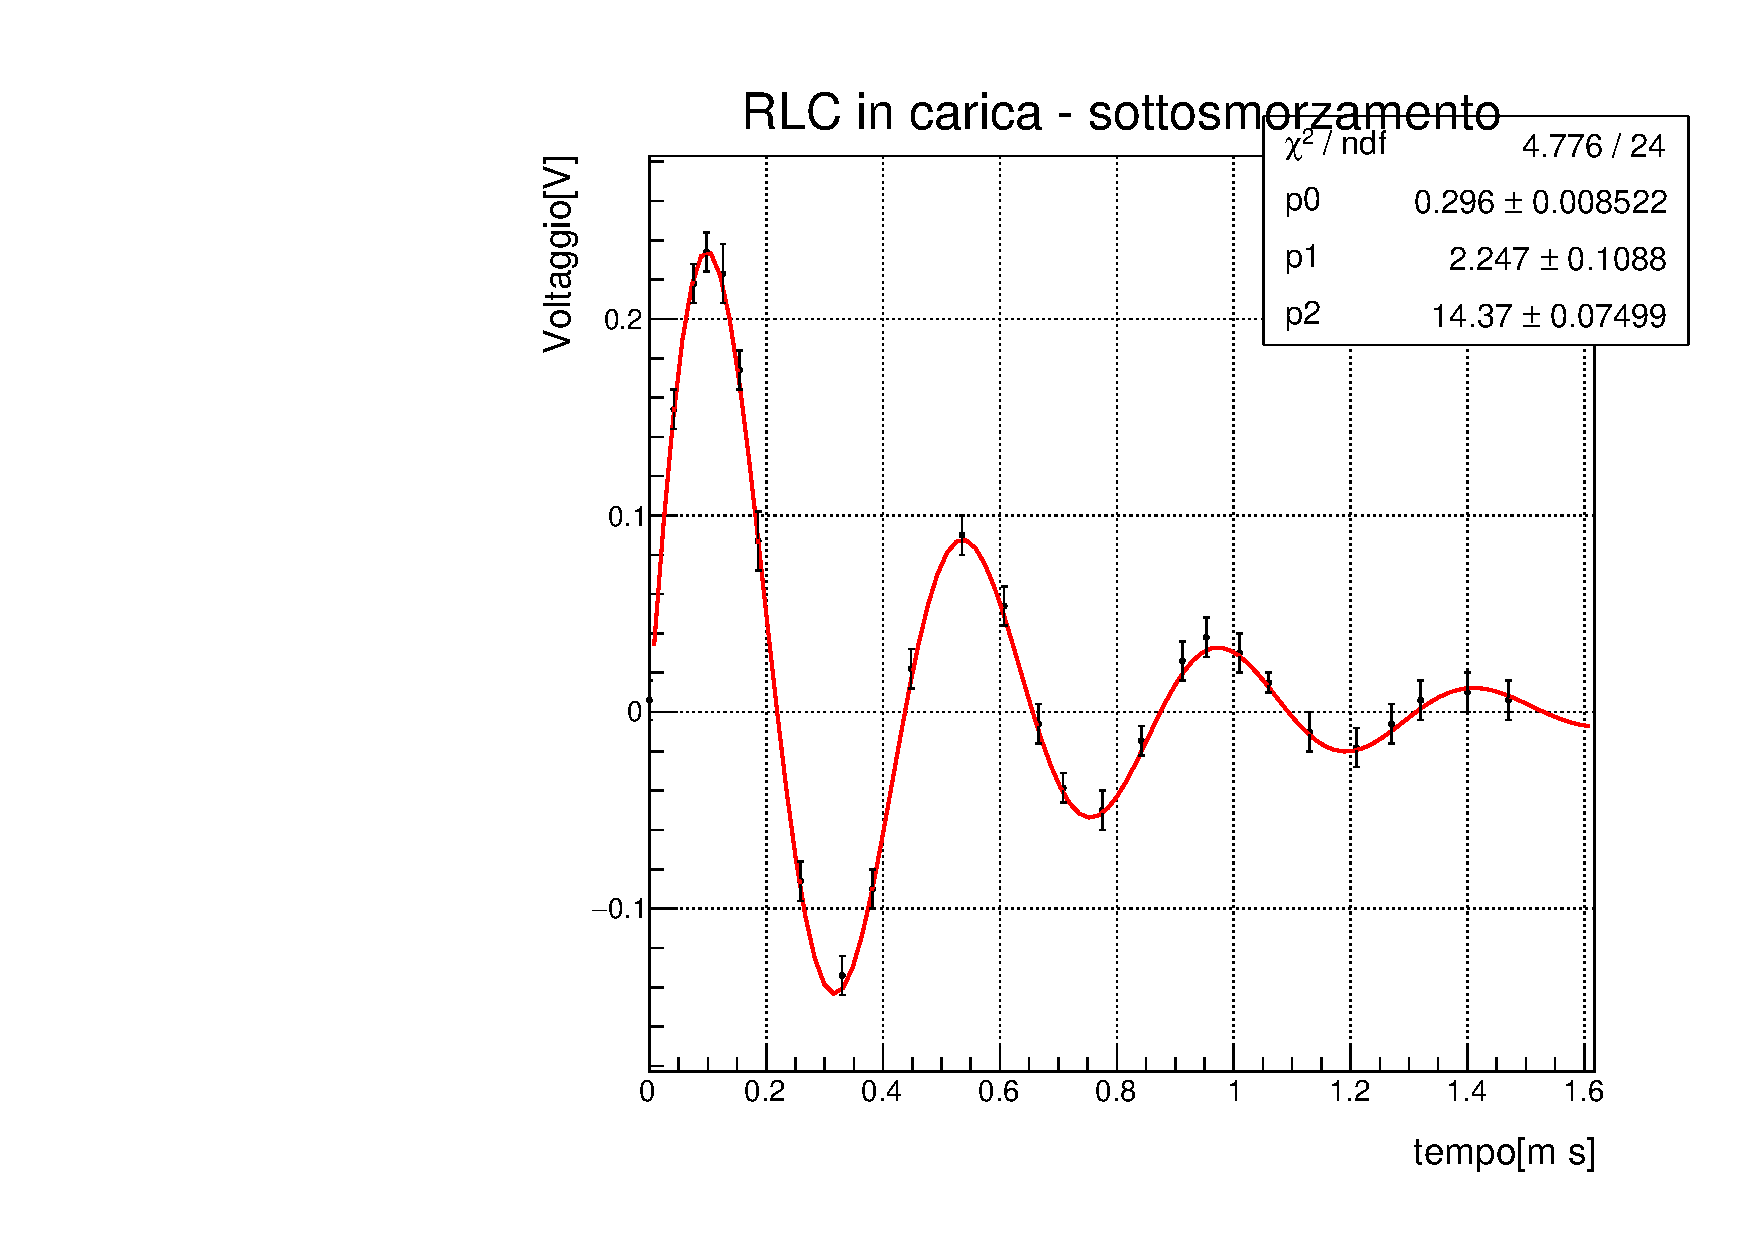
\includegraphics{seconda parte/sottosmorzamento.pdf} 
			}
	} %close centering
	\caption{funzione usata per l'interpolazione:  \(p_{0}e^{- x p_{1}}sin(xp_{2}) \) }

    \label{fig:sottosmorzamento}

\end{figure}
\noindent Il test del chi quadro suggerisce in questo caso una correzione negli errori associati alle misure di un fattore \(\frac{\chi^{2}}{Ndf} = 5\). \\

\noindent In termini di parametri, a seguito della correzione delle incertezze, abbiamo ottenuto \\

\( p_{0} = A \cdot R =  0.296  \pm 0.009  V \), che rappresenta la quota da cui l'esponenziale che domina il grafico comincia a decrescere; \\

\(p_{1} = \gamma  = \frac{R}{2\cdot L}= 2.2  \pm 0.1 ms^{-1} \) e \( p_{2} = \beta = \sqrt{\omega^{2}_{0} - \gamma^{2}} = 14.37  \pm 0.07 ms^{-1} \). \\

\noindent Osserviamo che il primo picco incontrato, il cui massimo corrisponde a \(\simeq 0.2V\), non corrisponde al picco che un circuito con i nostri parametri produrrebbe idealmente (si fa riferimento al grafico ottenuto con il software per la simulazione di circuiti elettronici NI Multisim), è bensì più basso. Una attenta analisi dei parametri in gioco permette di notare un errore increscioso nella scelta della resistenza, così piccola da essere paragonabile alle resistenze parassite del circuito di cui abbiamo effettuato una stima nella sezione \nameref{subsec:res_parassite} relativa al \nameref{sec:circuitoRL}. Dovremo dunque tenere conto, almeno per questa scelta di R, di una resistenza equivalente \(R_{eq}  = R + R_{par} \neq R\). \\
\noindent Possiamo calcolare \(\tau = \frac{1}{\gamma \cdot 2}\pm \frac{\sigma_{\gamma}}{2\gamma^{2}}\) e ottenere un'altra stima di L per controllare che si accordi con la media pesata precedente. Con \(\tau\) in ms e \(R_{eq}\) in \(k \Omega\)

\[L = \tau \cdot  R_{eq}=  0.051  H \]
\[\sigma_{L} = \sqrt{(\sigma_{\tau}  R_{eq})^{2} + ( \sigma_{R_{eq}} \tau  )^{2}} = 0.007  H\]
dunque L risulta pari a \( 51 \pm 7 H \). Abbiamo confrontato questo valore con la media pesata ottenuta per L tramite il test t-Student. 

\[t = \frac{\left|L_{3} - \bar{L} \right|}{\sqrt{\sigma^{2}_{L_{3}} + \sigma^{2}_{\bar{L}}}} = \frac{\left| 51 - 47.80734\right|}{\sqrt{7^{2} + 0.00008^{2}}} = 0.5 \rightarrow PValue = 61.71\%\]

\noindent Conoscendo \(\beta = 14.37 \pm 0.07 ms^{-1}\) possiamo anche ricavare \(C = \frac{1}{L \cdot \omega^{2}_{0}}\), tenendo in considerazione che \(\omega^{2}_{0}\) dipende anche da \(\gamma\) dunque la sua precisione dipende anche dalla correlazione tra le due \(\sigma_{\beta \gamma} = -9.122  \cdot 10^{-4}\). 

\[\omega^{2}_{0} =( \beta )^{2} + ( \gamma)^{2} = 211 ms\]
    \[ \sigma_{\omega^{2}} = \sqrt{  (2\beta\sigma_{\beta})^{2} + (2\gamma\sigma_{\gamma})^{2} + 2 \cdot 4 \beta \gamma \sigma_{\beta \gamma}  } = 2 ms\]
se \(\omega^{2}_{0}= 211.5 \pm 0.4\)ms allora:

\[\hat{C} = \frac{1}{L\omega^{2}_{0}} = 0.09 \mu F\]
    \[ \sigma_{\hat{C}} = \sqrt{ \left(\frac{\sigma_{L}}{L^{2}\omega^{2}_{0}}\right)^{2} +\left(\frac{\sigma_{\omega^{2}}}{(\omega^{2}_{0})^{2}L)}\right)^{2}  } =  0.01\mu F\]
    
    
\noindent concludiamo che \(C = 90 \pm 10 nF\), confrontandola con i 99\(\pm 1\) nF attesi otteniamo.

\[t = \frac{\left|C_{t} - \hat{C} \right| }{\sqrt{\sigma^{2}_{\hat{C}} + \sigma^{2}_{C_{t}}}}=\frac{\left| 99 - 90\right|}{\sqrt{1 + 10^{2}}} = 0.9 \rightarrow PValue = 36.81\%\]


\pagebreak

\subsection{Regime critico}
É possibile instaurare il cosiddetto regime critico di un circuito RCL nel caso in cui la scelta di R ricada in una buona approssimazione del valore \(\sqrt{\frac{4\cdot L}{C}}\) che noi siamo in grado di stimare a \(1.390 \pm 0.007 k\Omega\) per il nostro circuito. 

\subsubsection*{Dati raccolti}
Durante l'esperienza in laboratorio, la scelta di R è stata effettuata a partire da una stima preliminare per L che si è rivelata scarsamente accurata, difatti una resistenza di R = 1224.0 \(\Omega\) è alquanto inferiore rispetto al valore richiesto. Ci aspettiamo dunque che i dati raccolti, pur non presentando l'andamento tipico del regime in sottosmorzamento poichè R è dell'ordine di \(R_{critico}\), non saranno nemmeno compatibili con la forma funzionale dettata dal regime critico.\\

\noindent Si noti che abbiamo effettuato solo una misura per il voltaggio poichè il valore segnalato dall'oscilloscopio non variava, abbiamo dunque considerato la sensibilità dello strumento come errore sui valori, pari a 2mV.

\begin{table}[!htbp]


    \captionsetup{labelformat=empty}
    \caption{Tabella4: circuito LCR - regime "critico"}
\resizebox{11.5cm}{!}{

    \begin{minipage}{.5\linewidth}
      \caption{ }
      \centering
       \begin{tabular}{c|c}
        t[\(\mu\)s] & V [mV]  \\
        \hline
        \hline
        0.00& 0\(\pm 2\)\\
       \hline
       4.00& 176\(\pm 2\)\\
       \hline
       10.0& 424\(\pm 2\)\\
       \hline
       20.0& 752\(\pm 2\)\\
       \hline
       26.0& 904\(\pm 2\)\\
       \hline
       32.0& 1020\(\pm 2\)\\
       \hline
       38.0& 1120\(\pm 2\)\\
       \hline
       44.0& 1190\(\pm 2\)\\
       \hline
       52.0& 1260\(\pm 2\)\\
       \hline
       56.0& 1290\(\pm 2\)\\
       \hline
       64.0& 1310\(\pm 2\)\\
       \hline
       72.0& 1320\(\pm 2\)\\
       \hline
       80.0& 1310\(\pm 2\)\\
       \hline
       86.0& 1300\(\pm 2\)\\
       \hline
       92.0& 1270\(\pm 2\)\\
       \hline
       100& 1230\(\pm 2\)\\
       \hline
       110& 1180\(\pm 2\)\\
       \hline
       120& 1100\(\pm 2\)\\
       \hline
       130& 1040\(\pm 2\)\\
       \hline
       140& 968\(\pm 2\)\\
       \hline
       150& 888\(\pm 2\)\\
       \hline
       160& 816\(\pm 2\)\\
       \hline
       170& 752\(\pm 2\)\\
       \hline
       ... & ...\\
       \hline
       \hline
    \end{tabular}
    \end{minipage}%
    \begin{minipage}{.5\linewidth}
      \centering
        \captionsetup{labelformat=empty}

    	 \caption{ }
            \begin{tabular}{c|c}

        t[\(\mu\)s] & V [mV] \\
        \hline
        \hline
        
       ... & ...\\
       \hline
       80& 680\(\pm 2\)\\
       \hline
       190& 616\(\pm 2\)\\
       \hline
       200& 560\(\pm 2\)\\
       \hline
       210& 504\(\pm 2\)\\
       \hline
       220& 448\(\pm 2\)\\
       \hline
       230& 400\(\pm 2\)\\
       \hline
       240& 360\(\pm 2\)\\
       \hline
       250& 320\(\pm 2\)\\
       \hline
       260& 280\(\pm 2\)\\
       \hline
       270& 248\(\pm 2\)\\
       \hline
       280& 224\(\pm 2\)\\
       \hline
       290& 192\(\pm 2\)\\
       \hline
       320& 136\(\pm 2\)\\
       \hline
       340& 96.0\(\pm 2\)\\
       \hline
       360& 72.0\(\pm 2\)\\
       \hline
       380& 56.0\(\pm 2\)\\
       \hline
       400& 40.0\(\pm 2\)\\
       \hline
       420& 32.0\(\pm 2\)\\
       \hline
       440& 24.0\(\pm 2\)\\
       \hline
       460& 16.0\(\pm 2\)\\
       \hline
       480& 8.00\(\pm 2\)\\
       \hline
       500& 8.00\(\pm 2\)\\
       \hline
       540& 0.00\(\pm 2\)\\
        \hline
        \hline
    \end{tabular}
    \end{minipage} 
        }
        \caption{errore strumentale sui tempi: varia da \(\sigma_{t} = 0.02\mu\)s a \(2 \mu\)s}
        \label{tab_carica_RC}

\end{table}



\subsubsection*{Analisi dati e commenti}
L'interpolazione eseguita a partire dal modello atteso per I(t) in regime critico:
\[I(t)= At e^{-\gamma t}\]
ha prodotto il seguente risultato:


\begin{figure}[!ht]

	\makebox[1 \textwidth][c]{       %centering table
		\resizebox{0.70 \textwidth}{!}{   %resize table
			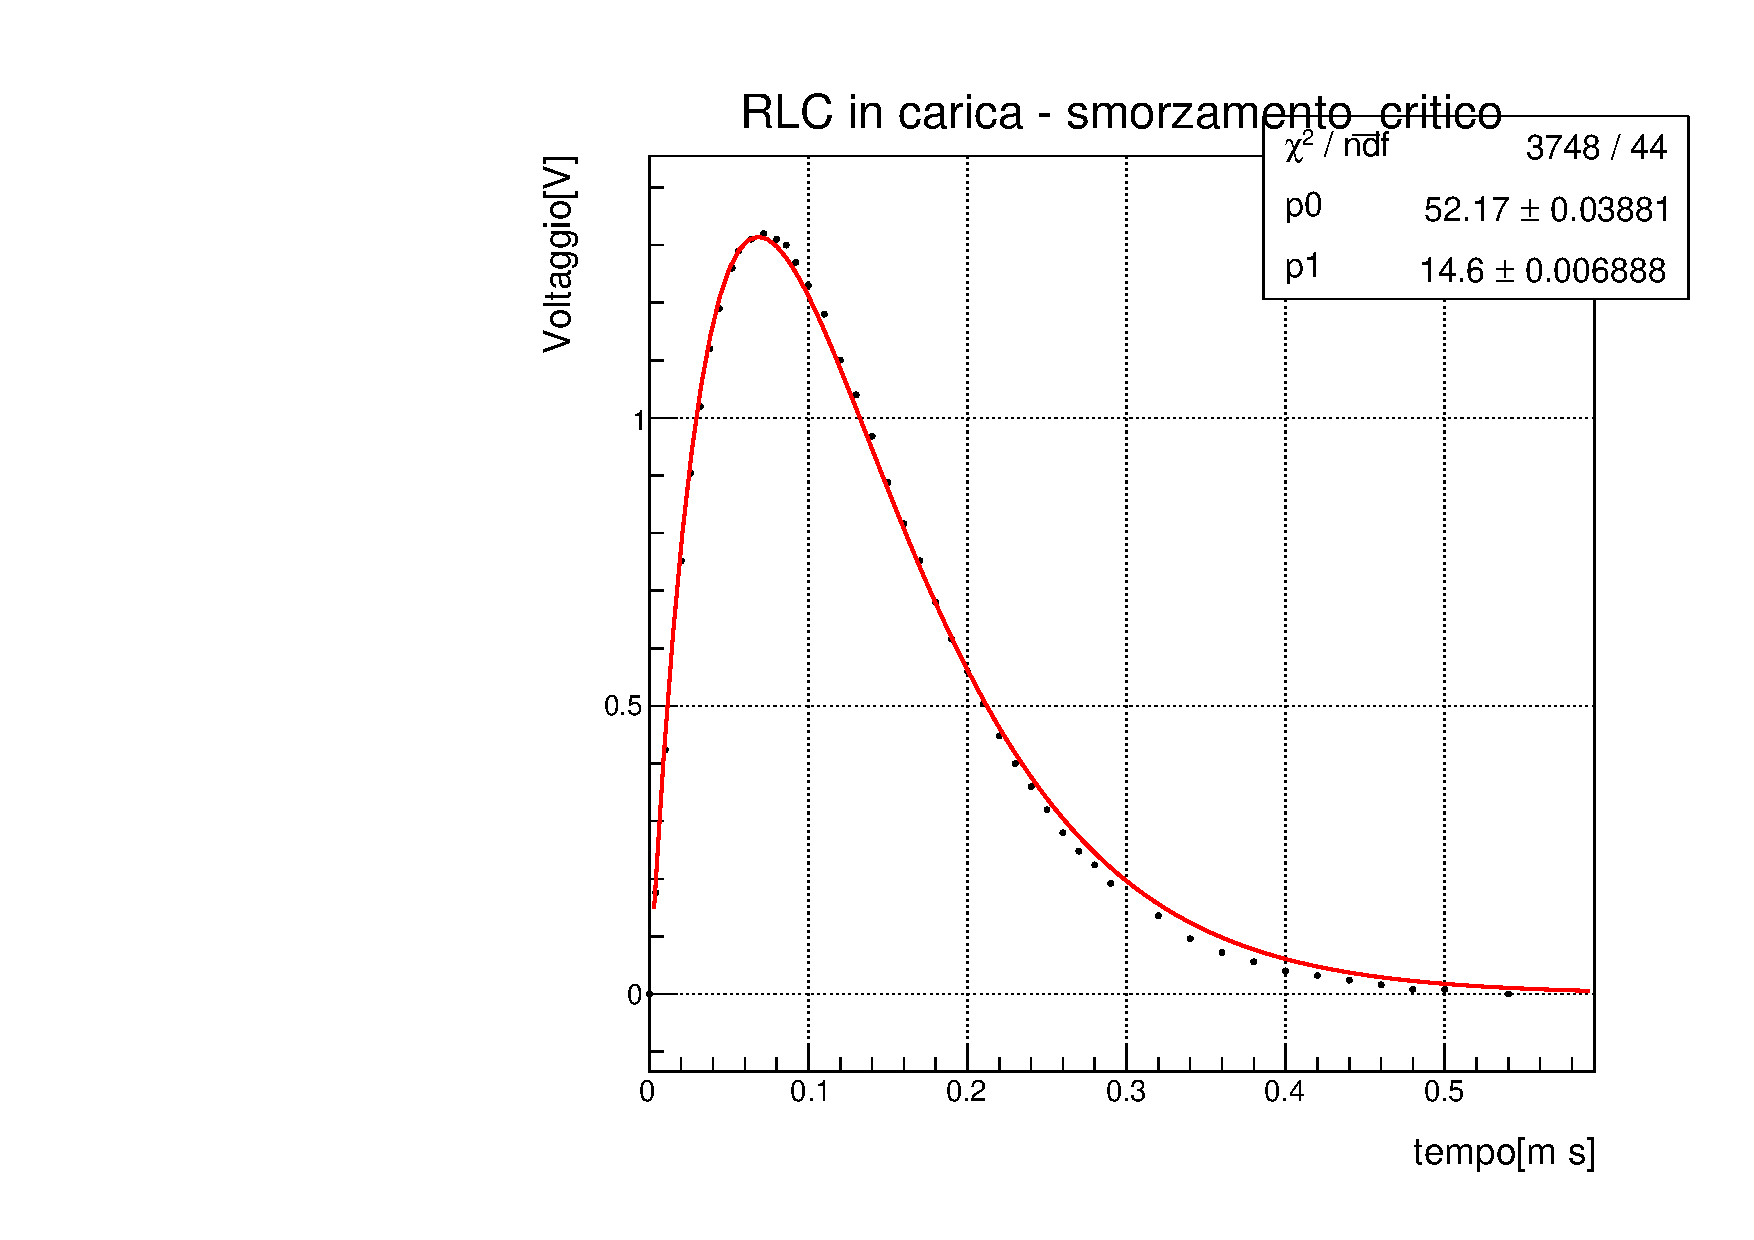
\includegraphics{seconda parte/smorzamento_critico.pdf} 
			}
	} %close centering
	\caption{funzione usata per l'interpolazione:  \(p_{0}xe^{-(p_{1}x)}\) }

    \label{fig:critico}

\end{figure}

\noindent Già dalla stima del \(\chi^{2}\)=3748 a confronto con il numero dei gradi di libertà Ndf = 44 possiamo notare che i dati non rispettano esattamente il modello atteso. Osserviamo infatti che l'andamento accenna l'instaurazione di un regime sottosmorzato, in cui la curva si abbassa rispetto all'asintoto a 0 per creare nuovi picchi. Per accertarci che la nostra ipotesi sia corretta abbiamo nuovamente eseguito il fit con la funzione attesa per il sottosmorzamento ed il chi quadro risulta in effetti \(\chi^{2} = 150.7\)/43 Ndf, un rapporto paragonabile a quello ottenuto già al paragrafo precedente. \\

\noindent I parametri riportati nella box assieme al grafico sono perciò poco significativi, li riportiamo di sotto per completezza \\

\(p_{0} = A = 52.17 \pm  0.04V \); \\

\(p_{1}  = "\gamma" = 14.600 \pm  0.007ms^{-1}\); mostriamo che se ricavassimo \(\tau\) come
  
\[\tau = \frac{1}{(2\gamma)} \pm \frac{\sigma_{\gamma}}{(2\gamma^ {2})}\] \\
tramite \(\tau\) in ms e R in k\(\Omega\) L risulterebbe \( L = 0.04192 \pm 2 \cdot 10^{-5} H\), la quale si dimostra essere incompatibile con la media pesata ottenuta precedentemente poichè
\[t = \frac{\left| \bar{L} - L_{3} \right|}{\sqrt{\sigma^{2}_{\bar{L}} + \sigma^{2}_{L_{4}}}} \approx 300 \rightarrow PValue = NA\]

\noindent In conclusione, per ottenere buoni risultati da questi dati avremmo dovuto procedere con un'analisi dati del tutto analoga a quella vista per il \nameref{subsec:sottosmorzamento}, che non riteniamo necessario riportare nuovamente. 

\pagebreak
\subsection{regime sovrasmorzato}

Per ottenere un regime sovrasmorzato è stato necessario scegliere un resistenza \(R > 1.305 k \Omega\). 

\subsubsection*{Dati raccolti}
Abbiamo selezionato una R = 1499\(\Omega\) misurata tramite il multimetro palmare; i dati raccolti tramite il campionamento sono riassunti nella tabella sottostante, anche questa volta i valori per V sono stati presi solo una volta quindi \(\sigma_{V} = 2\)mV per ogni misura.

\begin{table}[!htbp]
    \captionsetup{labelformat=empty}
    \caption{Tabella5: circuito LCR - regime sovrasmorzato}
\resizebox{12cm}{!}{

    \begin{minipage}{.5\linewidth}
      \caption{ }
      \centering
       \begin{tabular}{c|c}

        t[\(\mu\)s] & V [mV]  \\
        \hline
        \hline
        0.0 & 0\(\pm 2\)\\
        \hline
       10.0& 504\(\pm 2\)\\
       \hline
       20.0& 872 \(\pm 2\)\\
       \hline
       30.0& 1125 \(\pm 2\)\\
       \hline
       40.0& 1280 \(\pm 2\)\\
       \hline
       46.0& 1340 \(\pm 2\)\\
       \hline
       52.0& 1380 \(\pm 2\)\\
       \hline
       60.0& 1420 \(\pm 2\)\\
       \hline
       66.0& 1420 \(\pm 2\)\\
       \hline
       78.0& 1410 \(\pm 2\)\\
       \hline
       88.0& 1370 \(\pm 2\)\\
       \hline
       96.0& 1330 \(\pm 2\)\\
       \hline
       106& 1270 \(\pm 2\)\\
       \hline
       118& 1190 \(\pm 2\)\\
       \hline
       126& 1140 \(\pm 2\)\\
       \hline
       134& 1080 \(\pm 2\)\\
       \hline
       146& 1000 \(\pm 2\)\\
       \hline
       156& 936\(\pm 2\)\\
       \hline
       166& 872\(\pm 2\)\\
       \hline
       176& 808 \(\pm 2\)\\
       \hline
       186& 744\(\pm 2\)\\
       \hline
       196& 688 \(\pm 2\)\\
       \hline
       206& 640 \(\pm 2\)\\
       \hline
       216& 592 \(\pm 2\)\\
       \hline
       226& 544 \(\pm 2\)\\
       \hline
       236& 504 \(\pm 2\)\\
       \hline
       244& 464 \(\pm 2\)\\
       \hline
       256& 424 \(\pm 2\)\\
       ... & ...\\
       \hline
       \hline
    \end{tabular}
    \end{minipage}%
    \begin{minipage}{.5\linewidth}
      \centering
        \captionsetup{labelformat=empty}

    	 \caption{ }
            \begin{tabular}{c|c}

        t[\(\mu\)s] & V [mV] \\
        \hline
        \hline
        ... & ...\\
       266& 392 \(\pm 2\)\\
       \hline
       276& 360 \(\pm 2\)\\
       \hline
       286& 328 \(\pm 2\)\\
       \hline
       296& 304 \(\pm 2\)\\
       \hline
       306& 280 \(\pm 2\)\\
       \hline
       320& 248 \(\pm 2\)\\
       \hline
       336& 216 \(\pm 2\)\\
       \hline
       350& 192 \(\pm 2\)\\
       \hline
       366& 168 \(\pm 2\)\\
       \hline
       380& 152 \(\pm 2\)\\
       \hline
       396& 128 \(\pm 2\)\\
       \hline
       420& 104 \(\pm 2\)\\
       \hline
       438& 88 \(\pm 2\)\\
       \hline
       460& 72 \(\pm 2\)\\
       \hline
       480& 64 \(\pm 2\)\\
       \hline
       500& 56.0 \(\pm 2\)\\
       \hline
       520& 48.0 \(\pm 2\)\\
       \hline
       536& 40.0 \(\pm 2\)\\
       \hline
       560& 32.0 \(\pm 2\)\\
       \hline
       576& 24.0 \(\pm 2\)\\
       \hline
       590& 24.0 \(\pm 2\)\\
       \hline
       610& 24.0 \(\pm 2\)\\
       \hline
       636& 16.0 \(\pm 2\)\\
       \hline
       660& 16.0 \(\pm 2\)\\
       \hline
       676& 8.00 \(\pm 2\)\\
       \hline
       700& 8.00 \(\pm 2\)\\
       \hline
       720& 0.00 \(\pm 2\)\\  
        \hline
        \hline
    \end{tabular}
    \end{minipage} 
        }
        \caption{errore strumentale sui tempi: varia da \(\sigma_{t} = 0.2\mu\)s a 2 \(\mu\)s}
        \label{tab_carica_RC}

\end{table}







\subsubsection*{Analisi dati e commenti}

L'interpolazione eseguita a partire dal modello atteso per I(t):
\[I(t) = Ae^{-\gamma t} sinh(\beta t)\]
ha prodotto il risultato seguente:

\begin{figure}[!ht]
    \captionsetup{labelformat=empty}

	\makebox[1 \textwidth][c]{       %centering table
		\resizebox{0.70 \textwidth}{!}{   %resize table
			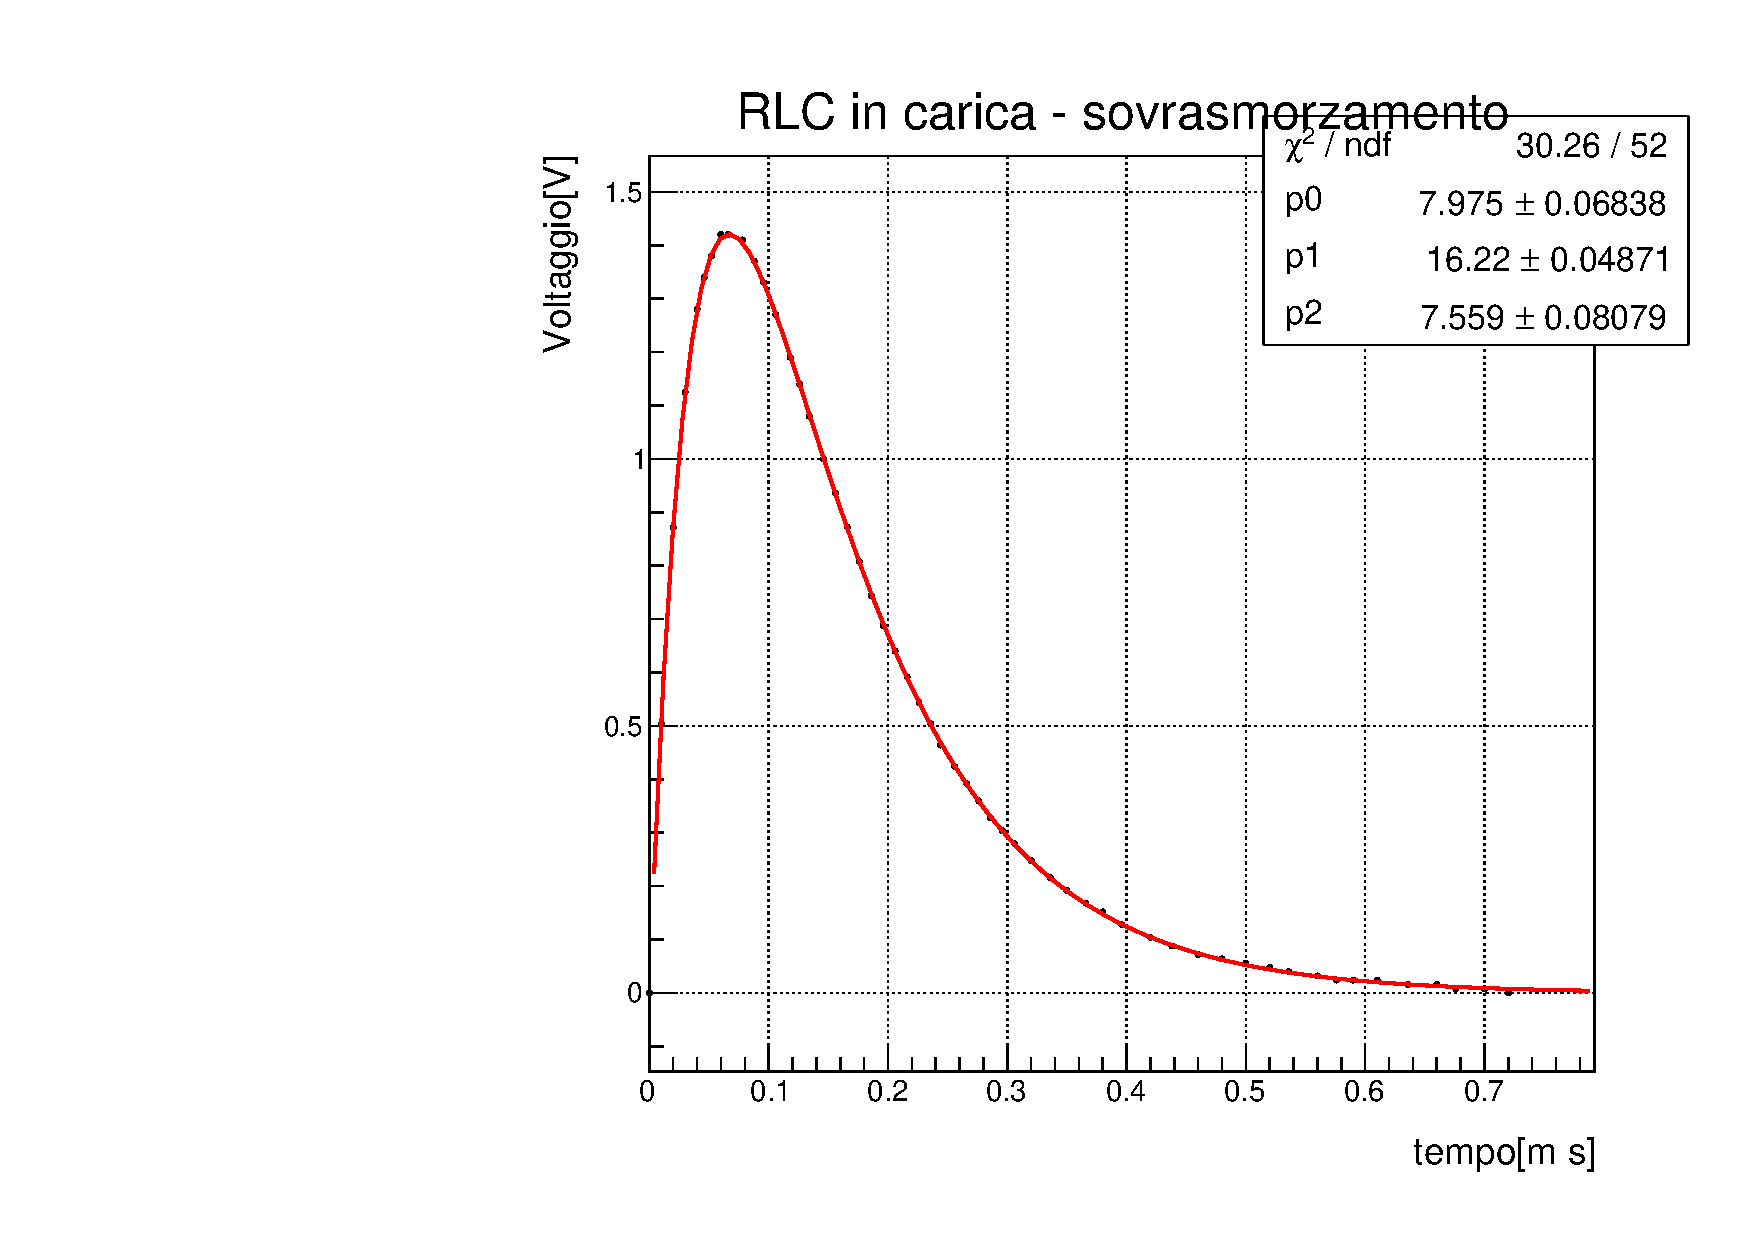
\includegraphics{seconda parte/sovrasmorzamento.pdf} 
			}
	} %close centering
	\caption{funzione usata per l'interpolazione:  \(p_{0}e^{-(xp_{1})}sinh(xp_{2})\) }

    \label{fig:sottosmorzamento}

\end{figure}

\noindent Sebbene ad un primo sguardo si noti che il grafico dei punti si adatta bene con il modello, il test del chi quadro rileva ancora una volta un errore nella stima delle incertezze: stimiamo che delle incertezze più realistiche per le nostre misure potrebbero essere pari a \(\sigma_{V} \cdot \frac{\chi^{2}}{Ndf} = 4 \)mV . \\

\noindent I risultati ricavati da ROOT per A, $\gamma$ e $\beta$ dopo aver corretto le incertezze sono: \\
 
\(  p_{0} =  A = 7.97  \pm 0.07V\), valore che regola l'altezza del picco della funzione; \\

\(p_{1}   = \gamma = 16.22 \pm  0.05 ms^{-1}\) e \(p_{2} = \beta = 7.56 \pm  0.08 ms^{-1} \). \\

\noindent Possiamo ora calcolare $\tau$ con \(\tau = \frac{1}{2\cdot \gamma} \pm \frac{\sigma_{\gamma}}{2\cdot \gamma^{2}} =  0.03082 \pm 5 \cdot 10^{-5} ms\) \\
 
\noindent e ottenere, con \(\tau\) in ms e R in k\(\Omega\),

\[L = \tau\cdot R =  0.0462 H \]
 \[\sigma_{L} = \sqrt{(\sigma_{\tau}\cdot R )^{2} + (\sigma_{R} \cdot \tau)^{2}} = 0.0001 H\]
 da cui segue la nostra miglior stima dell'induttanza: \(L = 46.2 \pm 0.1 mH \), la quale a confronto con la solita media pesata di \(\bar{L} = 47.80734 \pm 8 \cdot 10^{-5}\)mH, restituisce un t = 16, che corrisponde ad una probabilità di compatibilità così scarsa da essere inaccettabile. Per ottenere un risultato accettabile avremmo probabilmente dovuto stimare con più precisione gli errori sulle misure, che si dimostrano essere stati sottostimati. \\

\noindent Inoltre possiamo calcolare una nuova stima della capacità del condensatore: per farlo
sostituiamo \(\beta = 7.56 \pm  0.08 ms^{-1}\) e \(\gamma = 16.22 \pm  0.05 ms^{-1}\) nelle seguenti formule al fine di trovare $\omega$ 
\[\omega^{2} =\beta ^{2} + \gamma^{2}\]
\[ \sigma_{\omega^{2}} = \sqrt{  (2\beta\sigma_{\beta})^{2} + (2\gamma\sigma_{\gamma})^{2} + 2 \cdot 4 \beta \gamma \sigma_{\beta\gamma}   }\]
perciò se \( \omega^{2}= 320 \pm 2 \)ms, e usando l'induttanza ricavata in precedenza \(L = 46.2 \pm 0.1\)mH, la migliore stima per la capacità del condensatore sarà:

\[\hat{C} = \frac{1}{L\omega^{2}} = 0.0675694  \mu F \hspace{1cm}
\sigma_{\hat{C}} = \sqrt{ \left( \frac{\sigma_{L}}{L^{2}\cdot \omega^{2}} \right)^{2} +\left(\frac{\sigma_{\omega^{2}}}{(\omega^{2})^{2}L}\right)^{2}  } =   0.0005 \mu F\]

\noindent Da cui la nostra misura: \(C = 67.6 \pm 0.5 \) nF, che a confronto con \( 99 \pm 1 \) nF ricavata con il multimetro restituisce un t = 30, risultato ancora non accettabile. Osserviamo invece che questa stima per C risulta confrontabile con \(90 \pm 10\) nF ottenuto per il regime sottosmorzato per un t = 2 \(\rightarrow\) PValue = 4.6\%; supponiamo quindi che il valore segnalato dal multimetro non fosse accurato, siccome entrambe le stime che abbiamo ottenuto dai dati riportano valori inferiori del 10-30 \%.


\end{document}
